% interactcadsample.tex
% v1.03 - April 2017

\documentclass[]{interact}

\usepackage{epstopdf}% To incorporate .eps illustrations using PDFLaTeX, etc.
\usepackage{subfigure}% Support for small, `sub' figures and tables
%\usepackage[nolists,tablesfirst]{endfloat}% To `separate' figures and tables from text if required

\usepackage{graphicx}
\usepackage{multirow}
\usepackage[table]{xcolor}
\usepackage{adjustbox}
\usepackage{tabularx}
\usepackage[hidelinks]{hyperref}

\usepackage{natbib}% Citation support using natbib.sty
\bibpunct[, ]{(}{)}{;}{a}{}{,}% Citation support using natbib.sty
\renewcommand\bibfont{\fontsize{10}{12}\selectfont}% Bibliography support using natbib.sty

\theoremstyle{plain}% Theorem-like structures provided by amsthm.sty
\newtheorem{theorem}{Theorem}[section]
\newtheorem{lemma}[theorem]{Lemma}
\newtheorem{corollary}[theorem]{Corollary}
\newtheorem{proposition}[theorem]{Proposition}

\theoremstyle{definition}
\newtheorem{definition}[theorem]{Definition}
\newtheorem{example}[theorem]{Example}

\theoremstyle{remark}
\newtheorem{remark}{Remark}
\newtheorem{notation}{Notation}

\begin{document}

\articletype{Research Article}

\title{Reliability Conditions for Interpreting Daily NASA Black Marble
Nighttime Lights in Cloud-Impacted Tropical Regions}

\author{
\name{
Rene Jr. L. Principe\textsuperscript{a}
\thanks{CONTACT Rene Jr. L. Principe.
Email: s4135723@student.rmit.edu.au},
Karin Reinke\textsuperscript{a}
and Simon Jones\textsuperscript{a}
}
\affil{
\textsuperscript{a}Geospatial Science, School of Science,
STEM College, RMIT University, Melbourne, Victoria, Australia
}
}

\maketitle

\begin{abstract}
Satellite-derived nighttime lights (NTL) are widely used to infer electricity disruption and recovery following disasters, yet the conditions supporting reliable daily interpretation remain difficult to establish in persistently cloud-affected regions. Although NASA's Black Marble VNP46A2 product provides corrected daily radiance, cloud obstruction and quality screening create irregular observations, while spatial aggregation and temporal processing change the signal represented.

This study develops a diagnostic-first reliability-qualified NTL framework using Haiyan-affected Samar--Leyte, Philippines, as a demanding tropical test case. Spatial and temporal completeness, maximum dropout duration, and radiance variability are evaluated across nested pixel supports and Global Human Settlement Layer (GHSL) settlement classes. These diagnostics establish the observational context for cumulative GHSL masking, spatial-completeness thresholds, and alignment with independent electricity load across five Visayas sub-grids. Sensitivity analyses assess how configuration ranking and temporal averaging affect the resulting correspondence and observational support.

City- and municipal-centre groups retain admissible observations on approximately 29--34\% of days, while individual observation gaps reach 39 days. Spatial aggregation reduces radiance variability but provides little improvement in observational continuity. Urban-core masks are selected in four sub-grids, while Panay favours a broader urban-fringe mask, with selected completeness thresholds ranging from 5\% to 50\%. On directly paired daily observations, selected configurations yield correlations of $r=0.406$--$0.660$, retaining 27.7--56.9\% of available load dates across 1,216--2,495 paired days. Sensitivity tests show that exact selections depend on the ranking rule and that averaging can strengthen correspondence without increasing direct coverage. These findings demonstrate how spatial composition, observation gaps, and temporal processing jointly define the signal available for use. The framework provides a systematic basis for assessing whether the observational requirements of NTL disaster metrics are met in cloud-limited environments.
\end{abstract}

\begin{keywords}
VIIRS Day/Night Band; VNP46A2; spatiotemporal completeness;
observation gaps; electricity load; Philippines
\end{keywords}


\section{Introduction}

    Satellite-derived nighttime lights (NTL) provide one of the few globally consistent observational records of electrified human activity. Artificial illumination observed from space has been repeatedly shown to correlate with settlement presence, population distribution, infrastructure intensity, and economic output \citep{Elvidge1997,Chen2011,Henderson2012}. Since artificial lighting depends fundamentally on electricity access and consumption, satellite-measured nocturnal radiance offers a scalable proxy for the functioning of energy-dependent human systems. Unlike many socio-economic datasets that are spatially incomplete, administratively inconsistent, or temporally delayed, NTL observations are acquired systematically at global scale and have proven particularly valuable in data-constrained contexts where official statistics are sparse or lagged \citep{Jean2016,Tingzon2019,Zheng2023_ISPRSJPRS_UrbanReview,Levin2025_RSE_NTL_Agenda}.
        
    The systematic use of NTL in Earth observation began with the Defense Meteorological Satellite Program’s Operational Linescan System (DMSP–OLS). Early studies demonstrated that DMSP nightlight composites could delineate urban extents and approximate the spatial distribution of human settlements \citep{Elvidge1997,Small2005_RSE_UrbanExtent}. Subsequent analyses leveraged DMSP data to estimate economic production and growth patterns \citep{Chen2011,Henderson2012} and to track multi-decadal urban expansion \citep{Small2005_RSE_UrbanExtent}. DMSP-derived radiance was also applied in disaster contexts, including tsunami impact assessment in Southeast Asia \citep{Gillespie2014_RSL_Tsunami} and analyses of settlement proximity shifts following major flood events \citep{Mard2018_SciAdv_FloodProximity}. However, DMSP–OLS suffered from well-documented limitations, including coarse spatial resolution ($\sim$2.7 km), 6-bit radiometric quantization, saturation in bright urban cores, blooming artifacts, and reliance on annual composites that suppressed short-term variability \citep{Small2005_RSE_UrbanExtent}. These constraints limited its suitability for detecting rapid infrastructure disruption or localized power loss. The launch of the Visible Infrared Imaging Radiometer Suite (VIIRS) aboard the Suomi National Polar-orbiting Partnership satellite marked a generational transition in nighttime remote sensing. The VIIRS Day/Night Band (DNB) provides radiometrically calibrated measurements with substantially improved dynamic range, enhanced stray-light correction, and consistent near-global daily coverage \citep{Miller2013_RS_VIIRS_DNB,Kyba2015_RS_HighResNight}. This advancement transformed NTL from an annually aggregated indicator into a temporally resolved measurement capable of capturing day-to-day changes in electrified systems. Daily VIIRS observations have since been used to monitor disaster-induced outages \citep{Zhao2018_RS_DisasterAssessment,Zhao2020_AppliedGeography_PR}, track grid restoration \citep{Roman2019_PLOSone_Maria}, and quantify societal disruption during the COVID-19 pandemic \citep{Elvidge2020_RS_COVID_China,Ghosh2020_RS_COVID_India,Stokes2022_SciRep_MENA_COVID}.

    NASA’s Black Marble Product Suite (VNP46 series) further refined NTL observations by introducing physically based corrections for bidirectional reflectance distribution function (BRDF) effects, lunar irradiance, atmospheric scattering, and sensor geometry \citep{Roman2018_RSE_BlackMarble}. In addition to these radiometric adjustments, Black Marble provides per-pixel quality flags and a gap-filling framework intended to mitigate cloud-induced data loss. These developments enabled increasingly quantitative applications of daily NTL for infrastructure disruption and recovery analysis. However, the observational reliability of daily NTL remains unevenly treated across the literature. Here, \textit{observability} refers to the extent to which radiance values correspond to direct clear-sky surface measurements rather than temporally propagated or interpolated estimates. The amount and temporal distribution of direct observations therefore need to accompany interpretation of the corrected radiance series \citep{Zhao2019_RS_Review,Zheng2023_ISPRSJPRS_UrbanReview,Levin2025_RSE_NTL_Agenda}.

    The availability of daily observations does not, however, imply that the resulting radiance series records only changes in human activity. VIIRS DNB radiance remains sensitive to viewing geometry, natural background illumination, atmospheric conditions, and spatially varying surface structure. Multi-temporal analyses have shown systematic anisotropy in artificial-light observations as satellite view angle changes, particularly within vertically complex urban environments \citep{Li2019_RSE_Anisotropy}. Natural-light variation can also affect the detection of faint artificial sources, although background-based corrections substantially reduce this variability \citep{Coesfeld2020_Sensors_NaturalLight}. More broadly, retrieval-level uncertainty remains associated with atmospheric correction, viewing geometry, surface reflectance, and cross-sensor consistency even after operational processing \citep{Wang2021_RSE_RetrievalUncertainty}. \citet{Tan2023_IJAEOG_SpatialUncertainty} further demonstrated that environmental and observational factors explain spatially varying proportions of daily radiance variability and that these effects differ between urban and rural settings. These studies show that radiometric stability and observation availability are related but distinct dimensions of NTL reliability.
    
    Existing studies address irregular daily observations through several distinct strategies. One is temporal aggregation, which exchanges event-scale detail for a more stable representation of longer-term conditions. NASA’s VNP46A3 and VNP46A4 products combine quality-screened VNP46A2 observations into monthly and annual composites stratified by viewing-angle category and snow condition, while retaining quality and observation-count information \citep{Wang2022_IEEE_MultiangleComposites}. Such products improve temporal representation for long-term and structural analyses, but necessarily change the temporal scale at which variation can be resolved. \citet{Zheng2022_RSE_TemporalCompositing} showed that alternative temporal compositing strategies can materially alter NTL magnitudes, spatial distributions, temporal trends, and relationships with downstream variables. The use of a temporally aggregated or smoothed series therefore does not simply remove noise; it defines which forms and durations of change remain observable. This distinction is consequential for disaster applications, where electricity disruption and early recovery may occur within the period absorbed by a monthly composite.
    
    Empirical studies illustrate considerable methodological variation in preprocessing workflows, treatment of observation gaps, and approaches to assessing data reliability. \citet{Roman2019_PLOSone_Maria} demonstrated a strong correspondence between BRDF-corrected radiance and electricity load after Hurricane Maria, establishing the credibility of Black Marble for the tracking of restoration at the territory level. Subsequent work has expanded methodological sophistication in modeling and scaling, including machine-learning approaches to gap-filled time series \citep{Chakraborty2023_RSE_AdaptiveModeling}, gap-aware decomposition techniques \citep{Jia2023_IJAEO_ImprovedNTL_DisasterLoss}, and sensitivity analyses of recovery-duration estimates \citep{Zheng2025_RSE_InequalityRecovery}. 
    
    Electricity-focused applications have further strengthened the empirical basis for interpreting NTL as an indicator of power-system conditions across different spatial and temporal scales. \citet{Chakraborty2025_EF_ElectricityAccess} used a decade of Black Marble observations to map global electricity access and persistent electrification gaps at 1 km resolution, while \citet{Yang2026_Energy_UrbanRuralElectricity} integrated NTL, prefecture-level electricity consumption, and GHSL classes to produce settlement-stratified consumption estimates at 500 m resolution. At shorter temporal scales, \citet{Li2026_JGSA_SouthAfricaReliability} related monthly VIIRS-derived dispersion, anomaly, and seasonal indicators to electricity availability, outage shares, and load-shedding conditions in South Africa. \citet{Xu2026_RS_PowerReliability} developed a self-adaptive anomaly-detection framework for daily NTL and derived a satellite-based index that was evaluated against ground-measured grid reliability. For disaster recovery, \citet{Mo2025_ERIS_CycloneRecovery} estimated blackout durations following 396 tropical cyclones across 66 countries, validated NTL-derived durations against PowerOutage.US records, and represented periods without valid observations as uncertainty intervals. Collectively, these studies establish that NTL can represent electricity access, consumption, reliability, outages, and recovery, but they do so using different temporal products, validation targets, and processing assumptions \citep{Zhao2019_RS_Review,Levin2025_RSE_NTL_Agenda}. Proxy relevance and observational admissibility must therefore be treated as separate questions.

    A parallel body of work treats unavailable observations primarily as a reconstruction problem. \citet{Hao2023_GRS_BlackMarbleGapFilling} combined spatiotemporal weighting with bidirectional recurrent modelling to predict missing daily Black Marble values, while \citet{Tan2023_RSE_CRYSTAL} developed the CRYSTAL method to reconstruct cloud-obscured daily NTL by integrating spatial and temporal information from partially clear imagery. In the wider optical remote-sensing literature, spatial-spectral random forests similarly exploit neighbouring and multispectral information to predict cloud-obscured pixels \citep{Wang2022_SRS_SSRF}. These approaches make important contributions by improving the completeness and predictive accuracy of reconstructed image sequences. Their objective nevertheless differs from determining whether the original directly observed record provides sufficient support for a specific inference. Reconstruction produces model-derived values for unavailable dates, whereas observability concerns the direct measurements supporting interpretation. A reconstructed sequence may therefore be temporally complete without being continuously observed.
    
    These methodological distinctions are most consequential in persistently cloudy regions, where valid DNB-BRDF retrievals are irregular in both space and time. In humid tropical and monsoonal climates, coherent cloud systems can reduce valid-pixel support across extensive areas and produce prolonged observation gaps \citep{Zhao2019_RS_Review,Skoufias2021_GNHR_VIIRS_Hazards}. As a result, the number of directly observed measurements varies substantially across space and time. Recent disaster applications reflect different strategies for coping with this constraint. Some studies restrict analysis to a limited number of clear-sky observations to preserve interpretability \citep{Hu2025_UrbanClimate_FloodResilience}. Others rely on multi-day or monthly composites to extract seasonal or structural patterns, but at the cost of resolving short-lived outages or rapid recovery dynamics \citep{Mokhtari2025_SciRep_CoastalZones}. Although Black Marble’s gap-filling procedure improves nominal continuity \citep{Roman2018_RSE_BlackMarble}, it does not increase the number of directly observed clear-sky measurements. Consequently, hazard-impact inference remains sensitive to cloud persistence, filtering thresholds, and aggregation design \citep{Levin2025_RSE_NTL_Agenda,Zheng2023_ISPRSJPRS_UrbanReview}.

    Recent applications illustrate how observation limitations are commonly handled within event-specific preprocessing rather than evaluated as a primary result. For the 2023 Türkiye earthquakes, \citet{Levin2023_RS_TurkeyEarthquake} retained cloud-free VNP46A1 observations, compared pre- and post-event periods of different lengths, and reported dates for which no cloud-free pixels were available. The study demonstrated that carefully selected nightly observations can map acute earthquake impacts and recovery. Its event-specific design did not seek to establish transferable criteria for the amount or continuity of direct observation required for interpretation. Similarly, \citet{Zheng2022_RS_UkrainePower} used daily VNP46A2 radiance to identify conflict-related light reductions and estimate populations exposed to power shortages, while recognising background noise and the absence of field validation as limitations. COVID-19 studies used temporally aggregated VIIRS observations to detect sustained reductions in urban activity \citep{Elvidge2020_RS_COVID_China}, demonstrating the value of temporal smoothing for persistent changes but not necessarily for interruptions lasting only several days. These applications demonstrate the substantive value of NTL, but observational support is generally managed through date selection, temporal aggregation, uncertainty representation, or application-specific screening. It is less commonly evaluated as a separate upstream condition using a shared set of diagnostics.

    In addition to atmospheric constraints, settlement heterogeneity influences both the stability and interpretation of radiance. Dense urban centres typically exhibit persistent, high-intensity illumination, whereas peri-urban and rural settlements often display weaker signals and greater relative fluctuation \citep{Small2005_RSE_UrbanExtent}. The relationship between radiance and the human processes it represents is also spatially non-stationary. \citet{Wu2022_RS_SpatialHeterogeneity} found that roads, residential areas, commercial activity, and other urban features contributed differently to VIIRS radiance across locations and spatial scales. \citet{Martinez2023_RS_BlackMarbleSuitability} likewise showed that the suitability of daily gap-filled Black Marble radiance for population analysis varied with spatial and temporal aggregation. Together with the spatially heterogeneous uncertainty identified by \citet{Tan2023_IJAEOG_SpatialUncertainty}, these findings show that apparent radiance changes cannot be interpreted independently of settlement structure and analytical scale.

    Taken together, the literature reveals a methodological tension. Daily NTL are increasingly used as indicators of electricity disruption and recovery, yet the underlying observations are variously filtered, aggregated, smoothed, reconstructed, or modelled before interpretation. These procedures alter different properties of the signal. Assessing only the final processed series can obscure whether stronger correspondence arises from a different spatial target, a changed set of retained dates, or temporal averaging. A reliability assessment therefore needs to connect direct observability to spatial qualification and external correspondence, then evaluate averaging as a separate analytical choice. This distinction is particularly consequential in tropical cyclone regions, where infrastructure disruption can coincide with persistent cloud cover.
    
    Earlier work introduced reliability-qualified NTL and demonstrated that completeness screening and settlement stratification condition NTL--load alignment in the Visayas using temporally aggregated series \citep{Principe2026_ISPRS}. The present study develops this foundation into a systematic framework linking observation conditions, signal selection, and processing sensitivity.

    Using Samar--Leyte as the primary diagnostic region and evaluating alignment across five Visayas sub-grids (Figure~\ref{fig:Study Area}), the study makes three linked advances:
    
    \begin{enumerate}
        \item \textit{A systematic basis for qualifying NTL before interpretation.} The framework connects spatial support, completeness, observation gaps, and radiance variability to signal selection, establishing an ordered procedure for assessing the evidence available for event-period and longer-term analysis.
    
        \item \textit{Evidence that settlement composition determines the electricity-related signal.} GHSL-based comparisons show that urban-focused supports consistently favour daily NTL--load alignment, while preferred completeness thresholds vary across sub-grids. These results establish the need to evaluate spatial composition alongside observation availability.
    
        \item \textit{A separation of processing gains from observational support.} Ranking-rule and averaging-window tests establish how methodological choices affect the selected signal. Holding spatial settings and directly paired dates fixed reveals how averaging strengthens correspondence while leaving direct observation coverage unchanged.
    \end{enumerate}

    \begin{figure}[!htbp]
        \centering
        \makebox[\linewidth][c]{\includegraphics[width=1\linewidth]{figs/fig_01_study_area.png}}
        \caption{Study region and analysis units. (A) Locations of the five National Grid Corporation of the Philippines (NGCP) Visayas sub-grid service areas. (B) Samar--Leyte, the primary diagnostic region, with the ten points of interest (POIs) used for pixel-scale observability analysis. (C--F) Panay, Negros, Cebu, and Bohol sub-grids, respectively, used for cross-sub-grid NTL--load alignment assessment.}
        \label{fig:Study Area}
    \end{figure}
    
\section{Materials and Methods}

    \subsection{Study Region}
    
    The empirical focus of this study is the Samar--Leyte island group in Eastern Visayas, Philippines (Figure~\ref{fig:Study Area}). The region represents a stringent test environment for daily NTL analysis due to the concurrence of persistent tropical cloud systems and severe electricity disruption during Super Typhoon Haiyan in November 2013. Haiyan was one of the most powerful tropical cyclones ever recorded at landfall, affecting over 16 million people and causing widespread infrastructure damage across Eastern Visayas \citep{NDRRMC2014_Haiyan,UNISDR2015_Haiyan}. The event resulted in prolonged electricity outages, transmission failures, and system fragmentation across the Samar--Leyte sub-grid.
    
    More broadly, the Philippines is consistently ranked among the most disaster-exposed countries globally due to its geographic location along the Western Pacific typhoon belt and the Pacific Ring of Fire \citep{WorldRiskReport2023,UNDRR2022_GAR}. Frequent cyclones, high rainfall variability, and complex islanded grid structures create persistent challenges for optical satellite observability and infrastructure monitoring. These conditions make Samar--Leyte suitable for examining the observational requirements under which daily NTL can support interpretation of electricity-related dynamics.
    
    \begin{figure}[p]
        \centering
        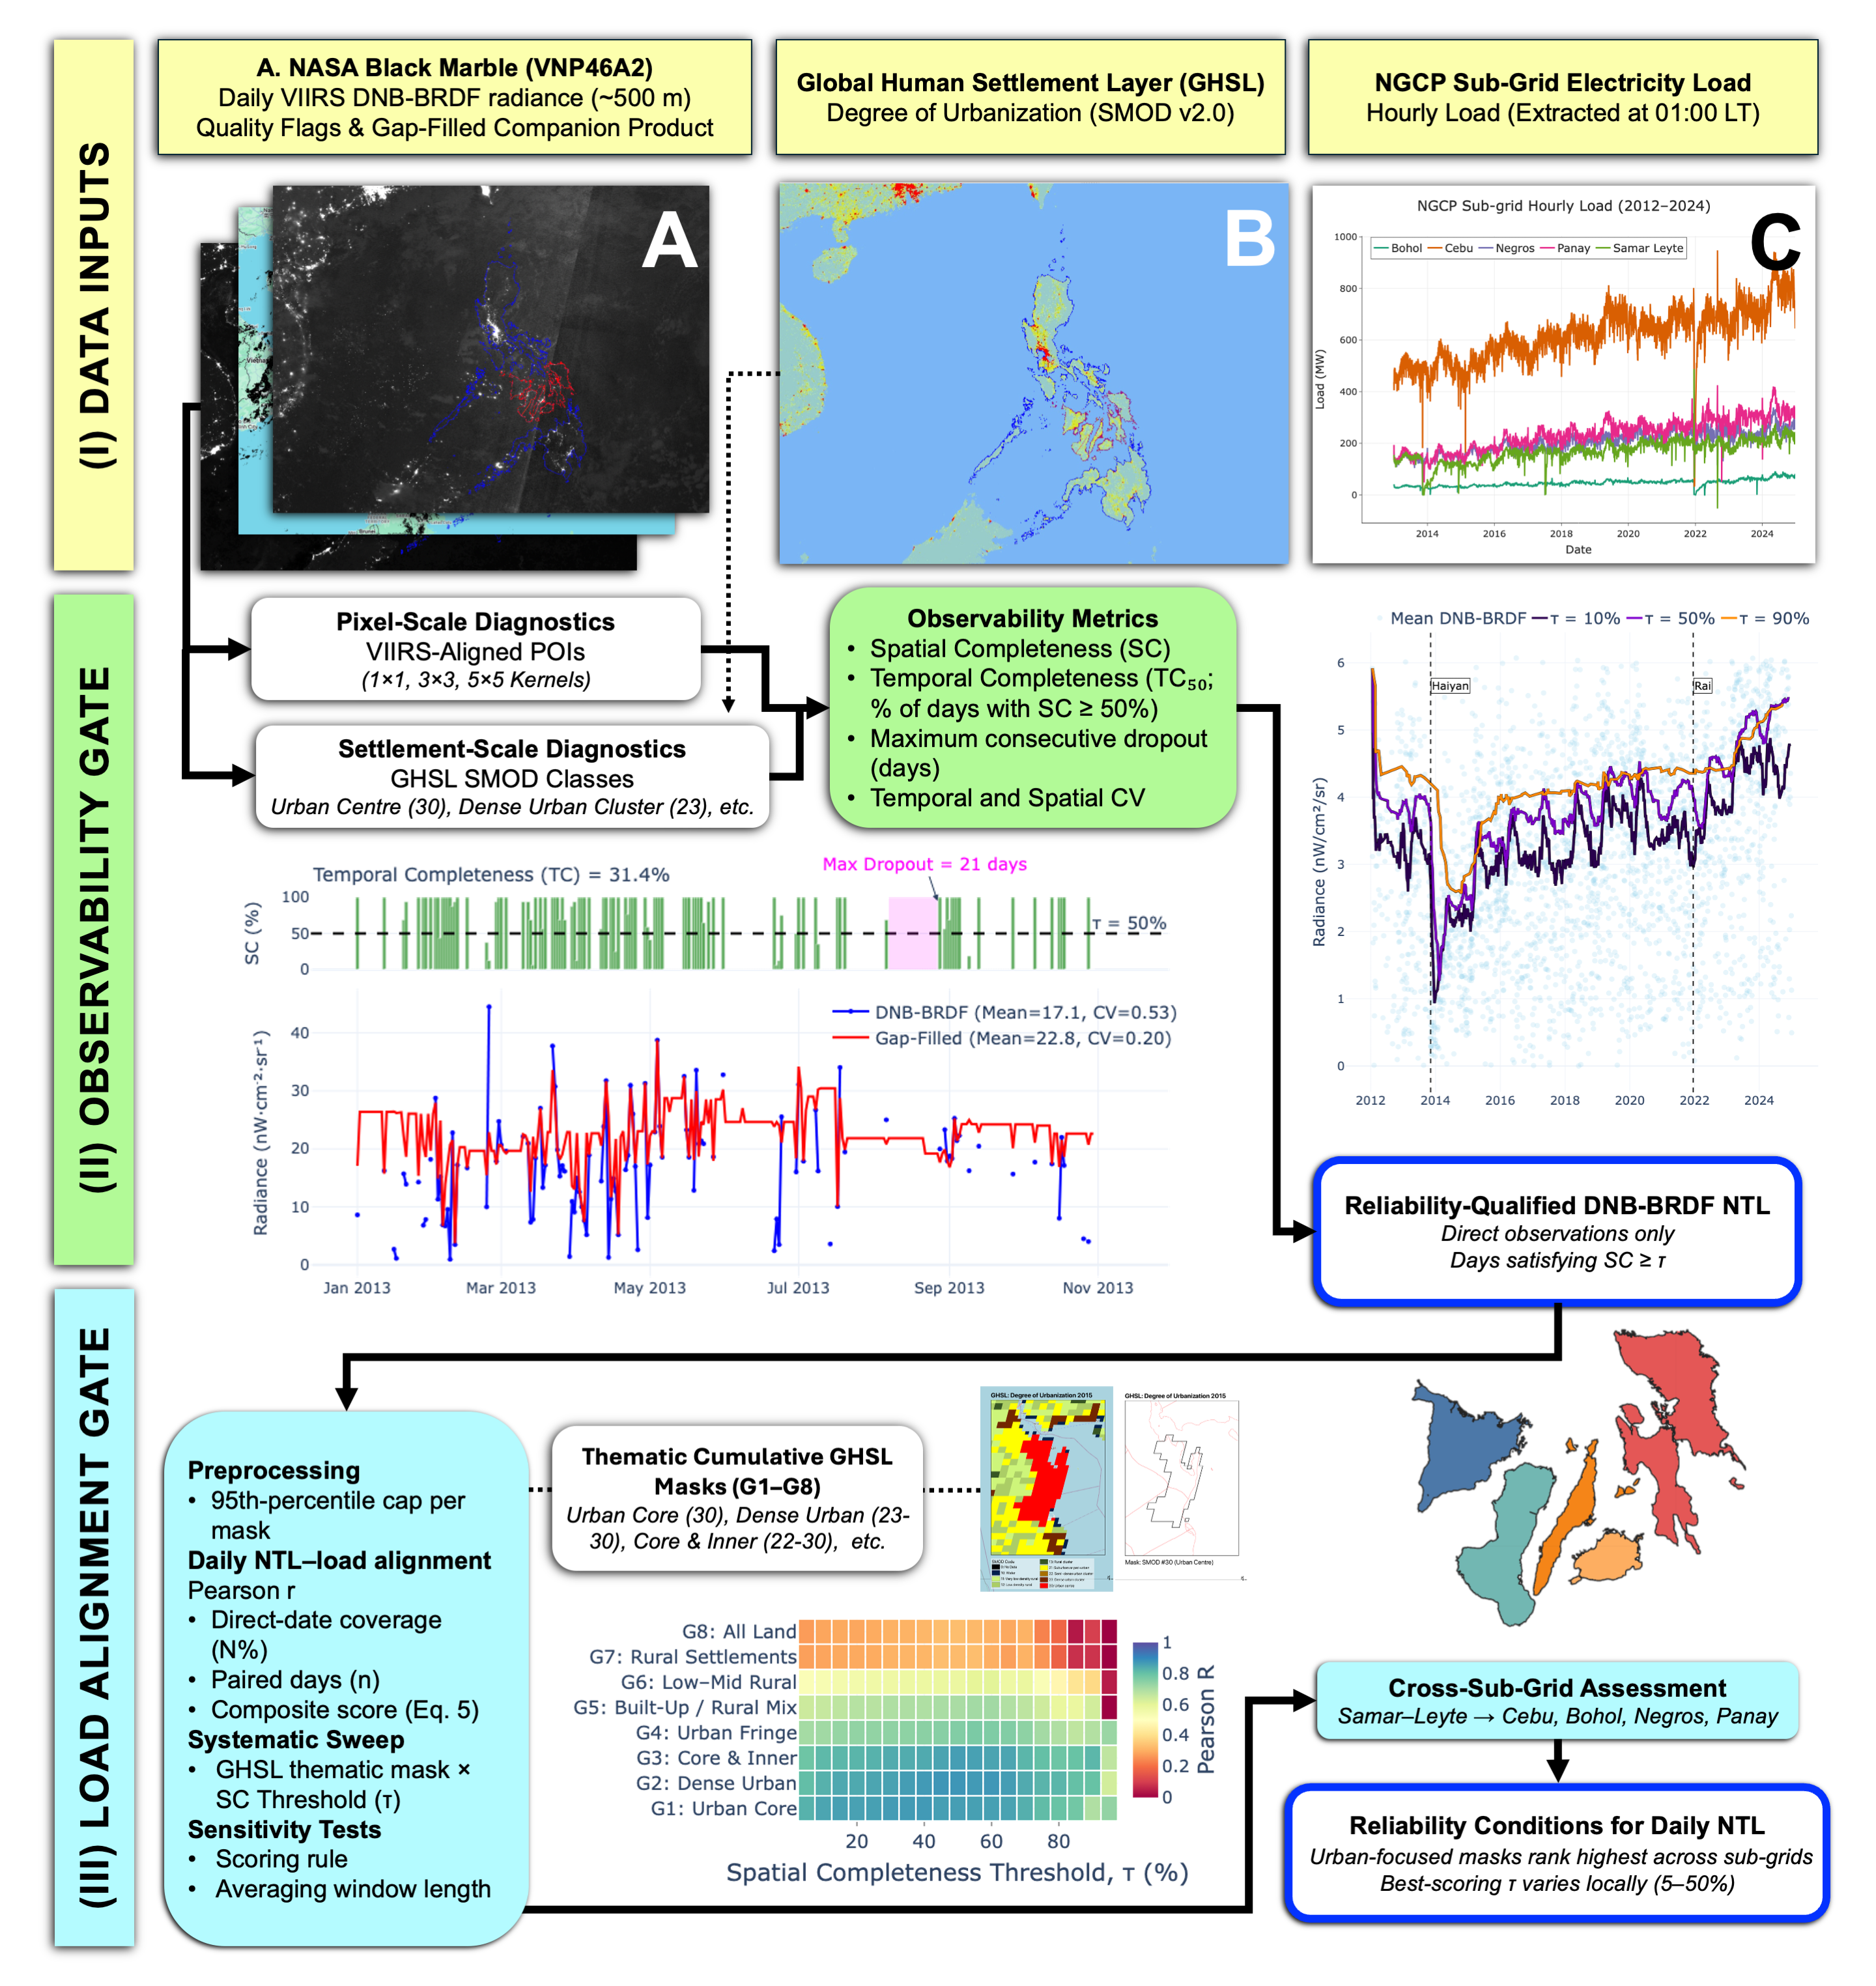
\includegraphics[
            width=\linewidth,
            height=1\textheight,
            keepaspectratio
        ]{figs/fig_02_schematic_diagram.png}
        \caption{Overview of the reliability-qualified NTL framework. Inputs comprise (A) NASA Black Marble VNP46A2 radiance, (B) Global Human Settlement Layer settlement classes, and (C) NGCP sub-grid electricity load. The workflow comprises observability diagnostics, spatial qualification, NTL--load alignment at $W=1$, within-sub-grid configuration selection, and sensitivity analysis of the scoring rule and temporal averaging.}
        \label{fig:schematic}
    \end{figure}
    
    Figure~\ref{fig:Study Area} situates the five Visayas sub-grids within the Philippine archipelago. Samar--Leyte contains ten points of interest (POIs) classified as city centres, municipal centres, and non-settlement references. The city-centre POIs are Tacloban, Ormoc, and Baybay; the municipal-centre POIs are Palo, Alang-Alang, and Guiuan; and the reference sites are Samar Forest Reserve, Mt. Nacolod Upland, Central Leyte Forest, and Southern Leyte Gulf. Site descriptions, coordinates, and selection rationale are provided in Supplementary Section~I and Table~S1. These POIs support examination of local NTL behaviour across contrasting illumination contexts and spatial supports before introducing settlement-based aggregation.
    
    The regional assessment extends to Panay, Negros, Cebu, and Bohol (Figure~\ref{fig:Study Area}C--F). These sub-grids provide contrasting island configurations and settlement structures within a demanding tropical observation environment. Independent electricity load records are available at the corresponding operational scale, allowing the same framework to examine how spatial support and observational availability condition NTL--load correspondence across the Visayas. The global temporal completeness assessment presented subsequently identifies the Philippines as a region of low daily observation availability.
    
    \subsection{Datasets}
    
    \begin{figure}[!t]
        \centering
        \subfigure[1 Nov 2013]{%
            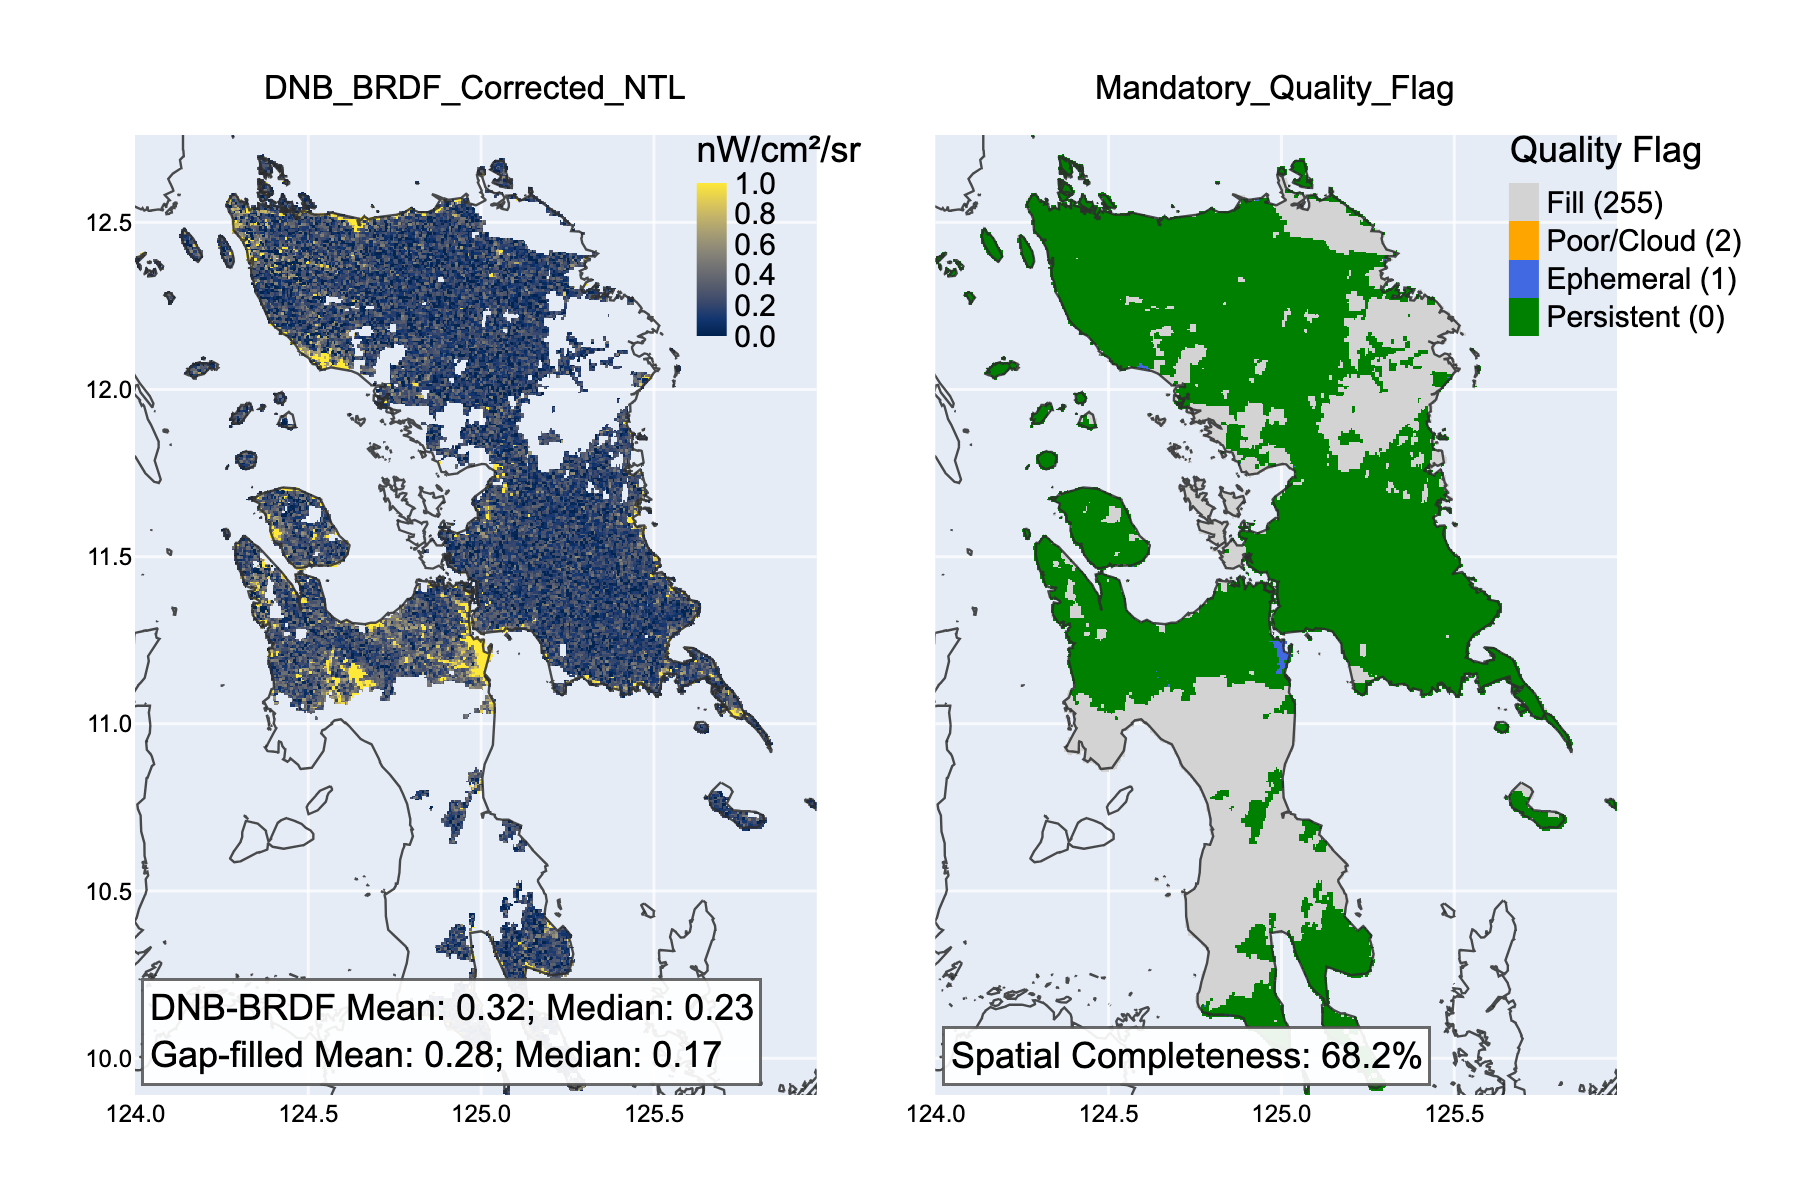
\includegraphics[width=0.48\linewidth]
            {figs/fig_03_20131101.png}
        }
        \hfill
        \subfigure[5 Nov 2013]{%
            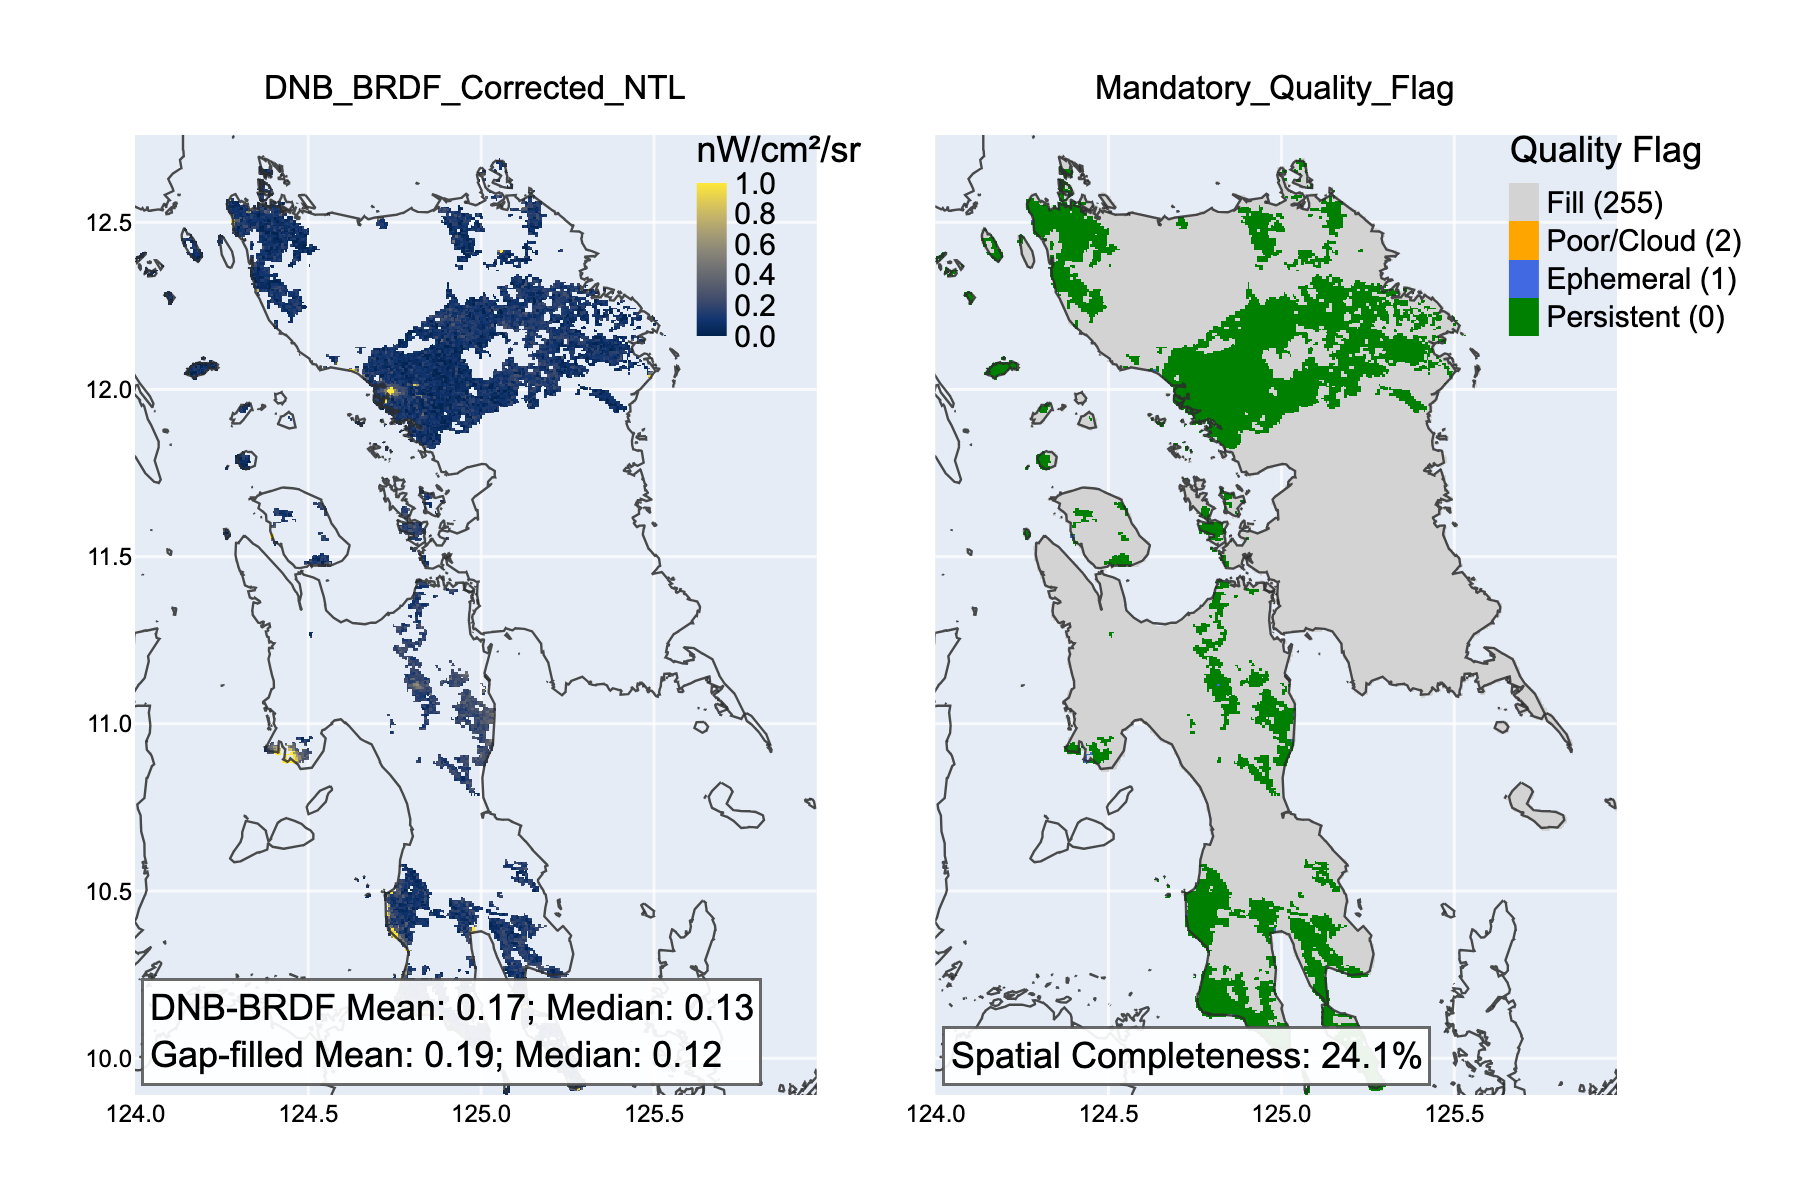
\includegraphics[width=0.48\linewidth]
            {figs/fig_03_20131105.png}
        }
    
        \par\medskip
    
        \subfigure[10 Nov 2013]{%
            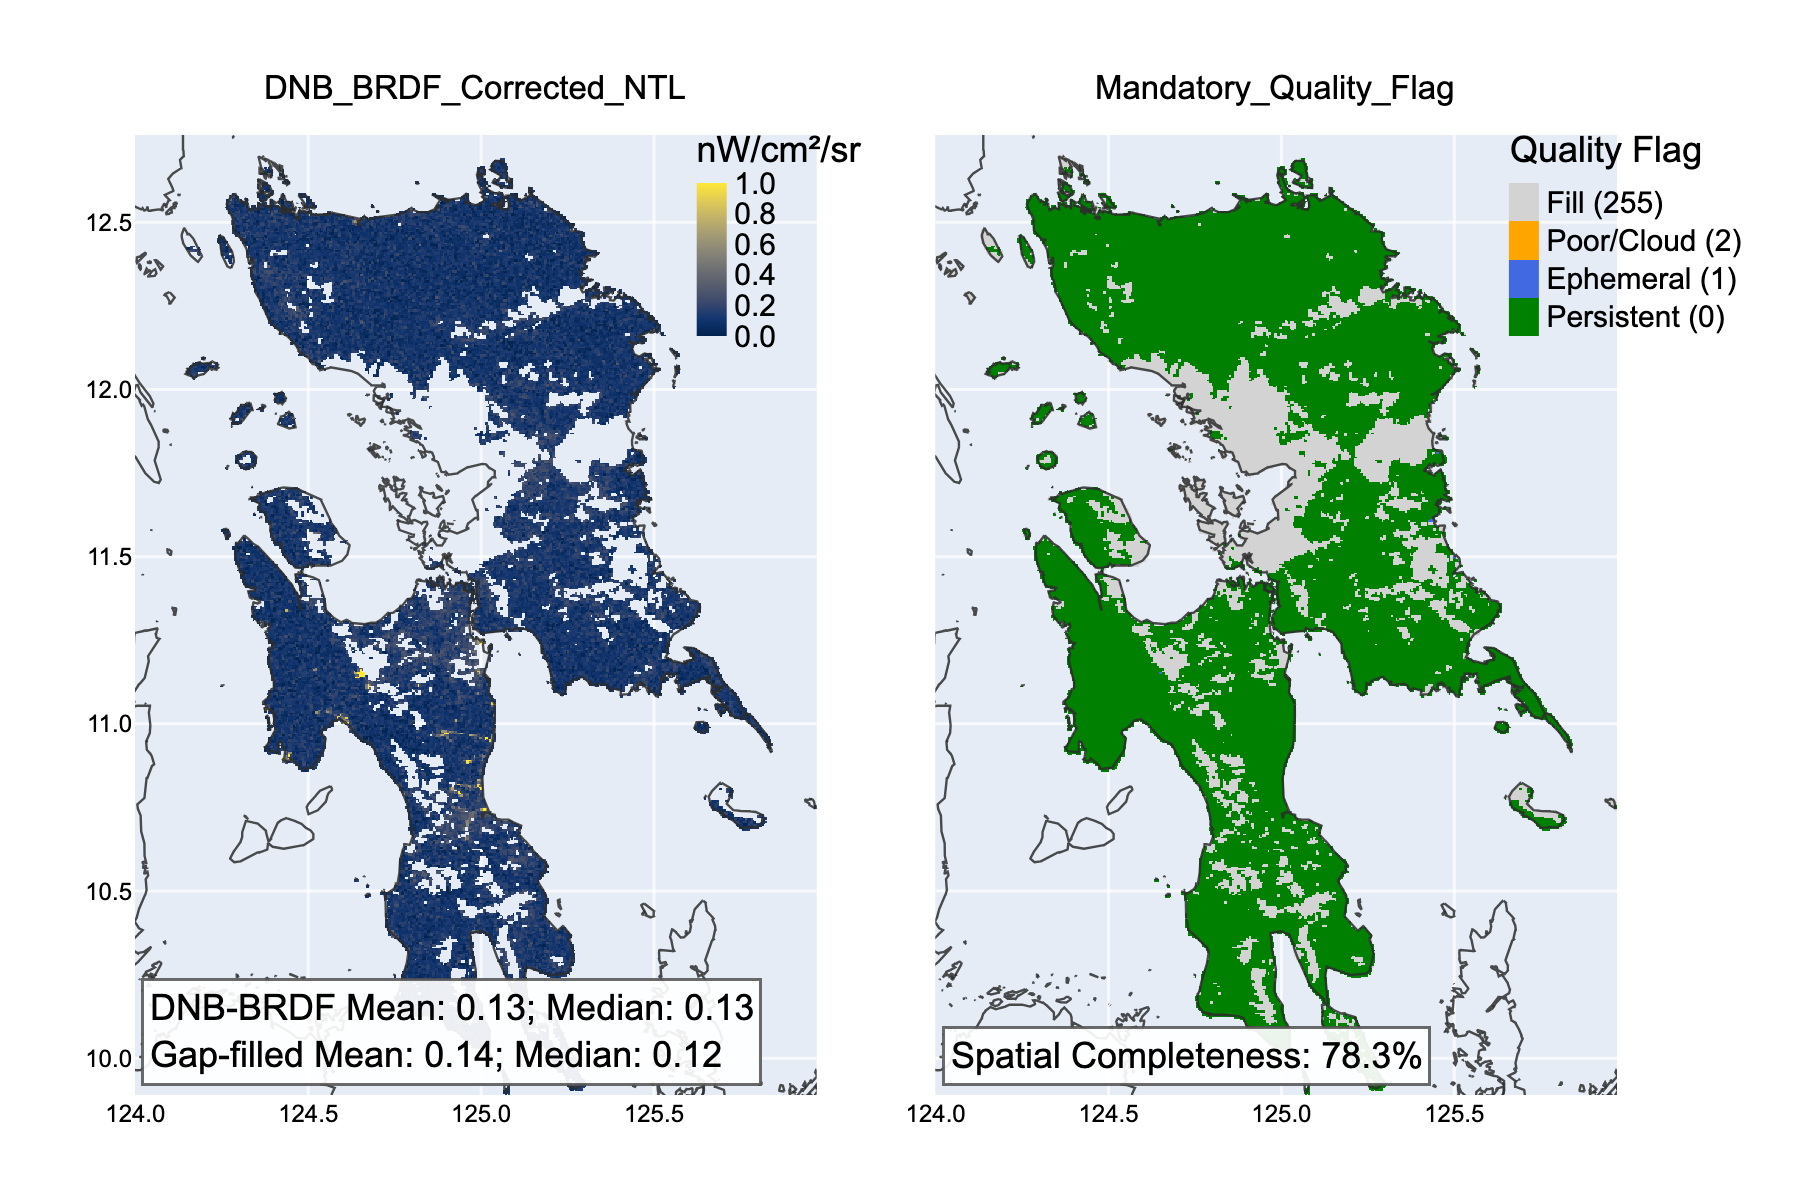
\includegraphics[width=0.48\linewidth]
            {figs/fig_03_20131110.png}
        }
        \hfill
        \subfigure[13 Nov 2013]{%
            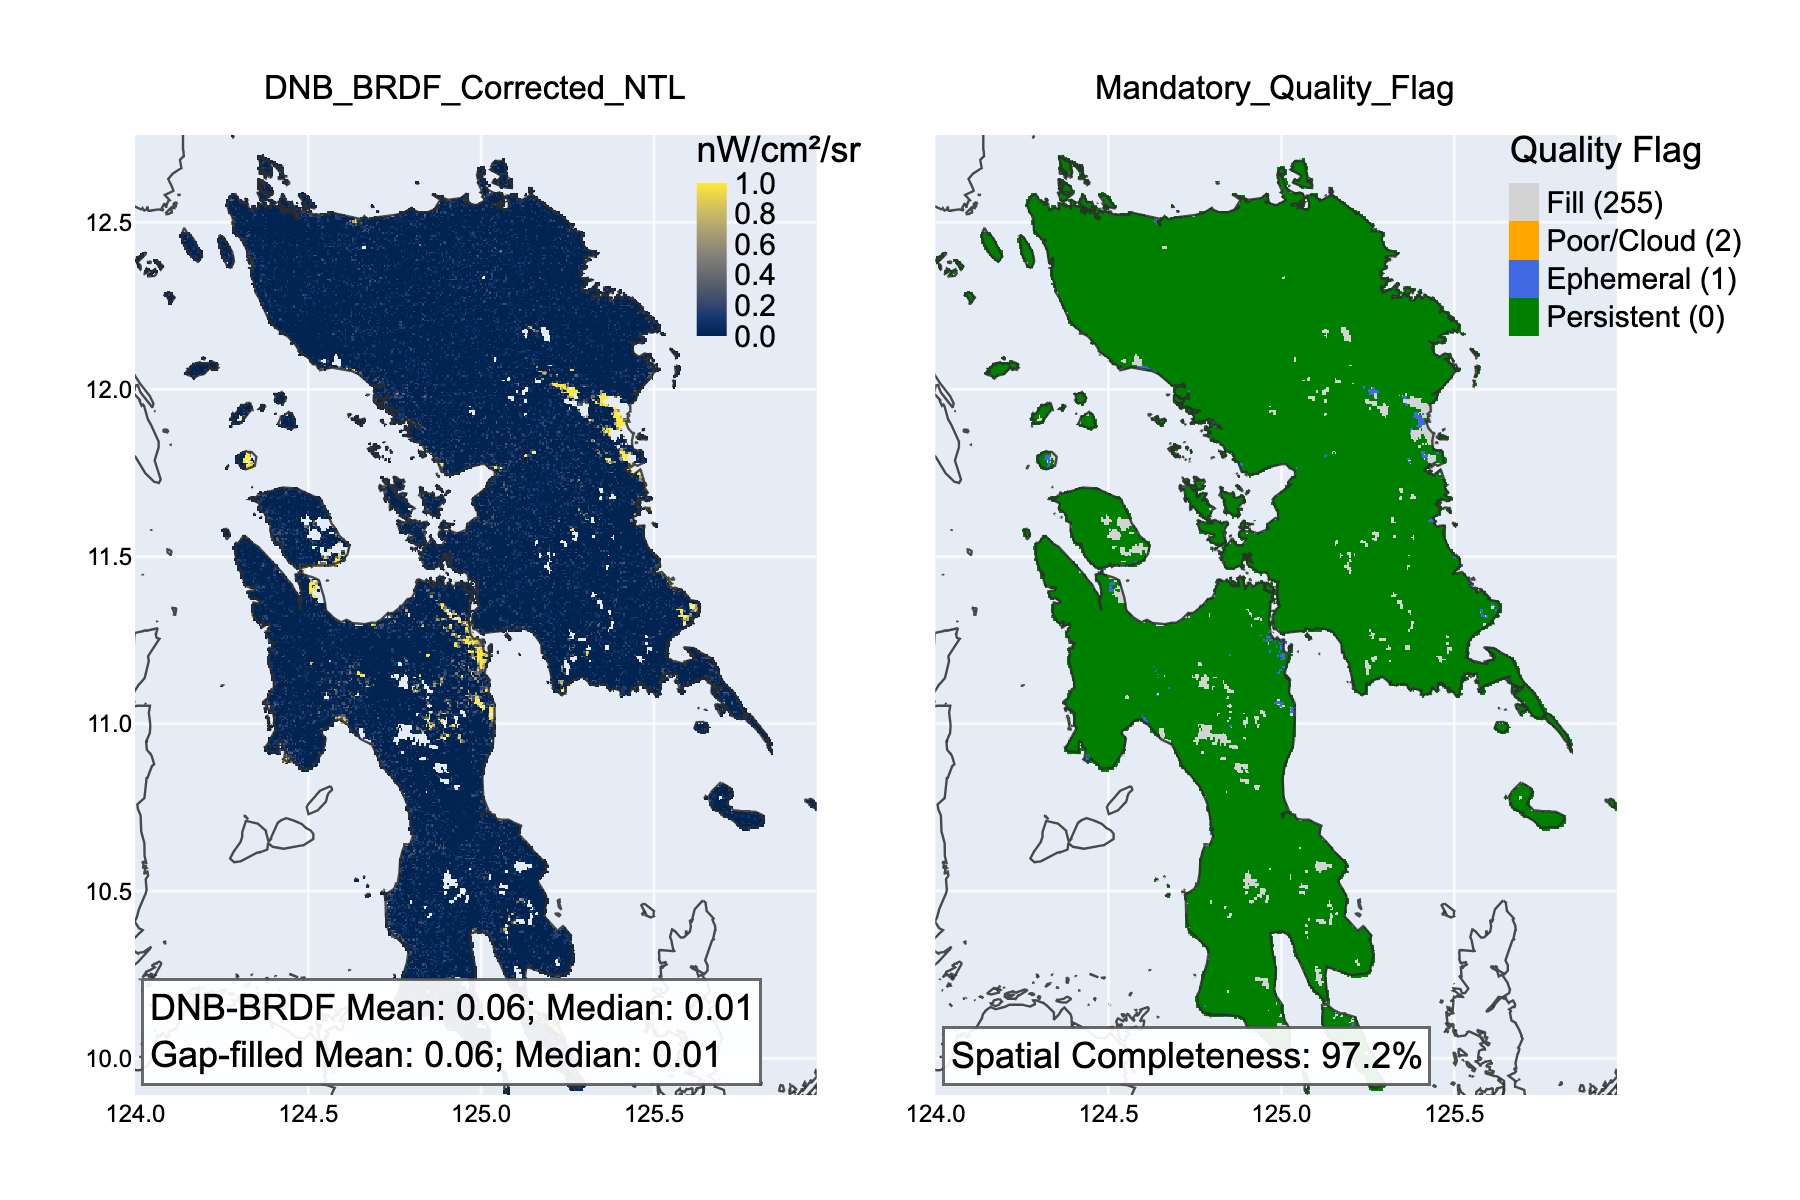
\includegraphics[width=0.48\linewidth]
            {figs/fig_03_20131113.png}
        }
    
        \caption{DNB-BRDF radiance and mandatory quality flags on 1, 5, 10, and 13 November 2013, bracketing Haiyan landfall on 8 November. Radiance is displayed using a common $0$--$1\,\mathrm{nW\,cm^{-2}\,sr^{-1}}$ colour scale, saturated at the upper limit. Annotations report mean and median radiance for the DNB-BRDF and gap-filled layers, and spatial completeness (SC), defined as the percentage of land pixels with valid DNB-BRDF retrievals.}
        \label{fig:fragmented_ntl}
    \end{figure}
    
    The analytical design integrates three data streams corresponding to Figure~\ref{fig:schematic}: (A) NASA Black Marble VNP46A2 radiance, (B) Global Human Settlement Layer (GHSL) settlement morphology, and (C) National Grid Corporation of the Philippines (NGCP) sub-grid electricity load. Datasets A and B support the observability diagnostics, while all three are integrated for NTL--load alignment. The POI and individual GHSL-class diagnostics use the 2013 calendar year. The longer 2012--2024 NTL record provides background information on observational availability and radiance dynamics, while load comparisons use the available NGCP reference dates during 2013--2024.
    
    Daily NTL observations (Figure~\ref{fig:schematic}A) are derived from NASA's Black Marble VNP46A2 Collection~2 product at approximately 500~m spatial resolution. Two radiance layers are examined: the BRDF- and lunar-corrected Day/Night Band radiance (DNB-BRDF) and its companion gap-filled layer. VNP46A2 observations intersecting the Samar--Leyte, Bohol, Cebu, Negros, and Panay sub-grid service areas were accessed through Google Earth Engine using \texttt{NASA/VIIRS/002/VNP46A2}.
    
    Direct DNB-BRDF observations were retained where \texttt{Mandatory\_Quality\_Flag} equalled~0 and the corresponding \texttt{QF\_Cloud\_Mask} conditions satisfied the adopted clear-sky screening rule. Pixels failing these conditions, including low-quality, cloud-contaminated, and fill observations, were treated as unavailable. The gap-filled layer is used for comparative diagnostics, while configuration selection uses quality-screened DNB-BRDF observations. Figure~\ref{fig:fragmented_ntl} illustrates the spatial discontinuities in direct coverage under persistent cloud systems, including over dense urban areas.
    
    \begin{table}[!h]
        \centering
        \footnotesize
        \setlength{\tabcolsep}{3pt}
        \tbl{GHSL SMOD v2.0 (GHS-SMOD R2023A), 2015 epoch, Level-2 settlement classes, classification criteria, and analytical groupings. The 2015 epoch provides a fixed settlement reference for the 2012--2024 analysis period. GHS-SMOD applies the Degree of Urbanisation methodology using population and built-up surface information from GHS-POP R2023A and GHS-BUILT-S R2023A \citep{Schiavina2023_GHSL_SMOD}.}{
        \begin{tabularx}{\linewidth}{l l >{\raggedright\arraybackslash}X l}
            \toprule
            \textbf{Code} &
            \textbf{Official Class} &
            \textbf{Degree of Urbanisation Criterion} &
            \textbf{Analysis Group} \\
            \midrule
            \cellcolor[HTML]{000000}\textcolor{white}{-200}
            & No Data
            & No valid settlement classification
            & Excluded \\
            \midrule
            \cellcolor[HTML]{7AB6F5}10
            & Water
            & $>50\%$ permanent surface water; not populated or built
            & Water \\
            \midrule
            \cellcolor[HTML]{CDF57A}11
            & Very low density rural
            & $<50$ inhabitants km$^{-2}$
            & \multirow{3}{*}{Non-urban Cells} \\
            \cellcolor[HTML]{ABCD66}12
            & Low density rural
            & $\geq50$ inhabitants km$^{-2}$; not part of a rural cluster
            & \\
            \cellcolor[HTML]{375623}\textcolor{white}{13}
            & Rural cluster
            & Contiguous cells; $\geq300$ inhabitants km$^{-2}$; cluster population 500--4,999
            & \\
            \midrule
            \cellcolor[HTML]{FFFF00}21
            & Suburban or peri-urban
            & Urban-cluster cells not belonging to an urban centre, dense urban cluster, or semi-dense urban cluster
            & \multirow{3}{*}{Urban Cluster} \\
            \cellcolor[HTML]{A87000}\textcolor{white}{22}
            & Semi-dense urban cluster
            & Contiguous cells; $\geq300$ inhabitants km$^{-2}$; $\geq5,000$ population; $\geq3$ km from dense urban clusters or urban centres
            & \\
            \cellcolor[HTML]{732600}\textcolor{white}{23}
            & Dense urban cluster
            & Contiguous cells; $\geq1,500$ inhabitants km$^{-2}$; cluster population 5,000--49,999
            & \\
            \midrule
            \cellcolor[HTML]{FF0000}\textcolor{white}{30}
            & Urban centre
            & Contiguous cells; $\geq1,500$ inhabitants km$^{-2}$; cluster population $\geq50,000$
            & Urban Centre \\
            \bottomrule
        \end{tabularx}
        }
        \label{tab:smod}
    \end{table}
    
    Settlement morphology (Figure~\ref{fig:schematic}B) is characterised using the GHSL Degree of Urbanisation Settlement Model (SMOD), release R2023A, version~2.0, produced by the European Commission Joint Research Centre \citep{Schiavina2023_GHSL_SMOD}. GHSL SMOD is provided at 1~km spatial resolution and classifies grid cells into a globally harmonised hierarchy of settlement types derived from population and built-up surface information. The 2015 epoch is held fixed throughout the analysis to maintain a consistent reference geography.
    
    For the observability diagnostics, individual SMOD Level-2 classes are evaluated separately and summarised within three analytical groups: Urban Centre (code~30), Urban Cluster (codes~21--23), and Non-urban Cells (codes~11--13), with Water (code~10) retained separately (Table~\ref{tab:smod}). For NTL--load alignment, these classes are combined into eight nested cumulative thematic masks, G1--G8. G1 contains only class~30; successive masks add classes~23, 22, 21, 13, 12, 11, and~10, respectively. G8 represents the full included domain, including water. Supplementary Section~IX describes the cumulative masks.
    
    Hourly electricity load data (Figure~\ref{fig:schematic}C) were obtained from NGCP \citep{NGCP_HourlyDemand} for the five operational sub-grids. Daily load values are extracted at 01:00 Philippine local time to approximate the VIIRS nighttime overpass at approximately 01:30 local time. Within each sub-grid, the load record provides an independent reference for evaluating radiance aggregated across the cumulative GHSL masks.
    
    \subsection{Diagnostic Framework}
    
    The reliability-qualified framework follows five steps (Figure~\ref{fig:schematic}): (1) characterise observational availability and radiance variability; (2) construct settlement-stratified radiance series and apply spatial completeness thresholds; (3) evaluate NTL--load correspondence at $W=1$; (4) select mask--threshold configurations using correspondence and retained coverage; and (5) assess sensitivity to the scoring rule and temporal averaging. The observability diagnostics develop the first step using the radiance and settlement inputs in Figure~\ref{fig:schematic}A--B. Electricity load alignment develops the remaining steps by integrating the NGCP reference in Figure~\ref{fig:schematic}C.

    \subsubsection{Observability Diagnostics}
        
        Observability is evaluated during 2013, encompassing persistent tropical cloud cover and the disruption associated with Super Typhoon Haiyan. Two complementary spatial scales are examined. First, local diagnostics are conducted at ten pixel-aligned POIs spanning city centres, municipal centres, and non-settlement references (Figure~\ref{fig:Study Area}; Supplementary Table~S1). Each POI is evaluated using nested $1\times1$, $3\times3$, and $5\times5$ VIIRS kernels to examine how expanding the spatial support changes radiance variability, valid-pixel availability, and observation continuity. Second, settlement-scale diagnostics are calculated for the individual GHSL SMOD classes in Table~\ref{tab:smod}, representing contrasting illumination environments across the wider Samar--Leyte domain.
        
        Four complementary metrics describe observability: spatial completeness, temporal completeness, maximum consecutive dropout duration, and radiance variability. For analysis unit $u$ on day $t$, spatial completeness is defined as
        
        \begin{equation}
        SC_{u,t} = \frac{n_{u,t}^{\text{valid}}}{n_u},
        \end{equation}
        
        where $n_{u,t}^{\text{valid}}$ is the number of valid DNB-BRDF pixels after quality screening and $n_u$ is the fixed total number of pixels within the same spatial support and analysis grid. Annual mean SC includes all 365 days of 2013, assigning zero valid pixels to dates without observations. SC is expressed as a fraction in the equations and as a percentage in figures and tables.
        
        A day is admissible when $SC_{u,t}\geq\tau$. The principal temporal-completeness and dropout diagnostics use $\tau=0.5$, requiring at least half of the spatial support to be valid. This corresponds to one, five, and 13 valid pixels for the $1\times1$, $3\times3$, and $5\times5$ kernels, respectively. Settlement-class temporal completeness is additionally evaluated at $\tau=0.25$ and $0.75$.
        
        For analysis unit $u$, year $y$, and threshold $\tau$, temporal completeness is defined as
        
        \begin{equation}
        TC_{u,y}(\tau) =
        \frac{
            \sum_{t\in y}
            \mathbb{I}\!\left(SC_{u,t}\geq\tau\right)
        }{
            n_y
        },
        \label{eq:temporal_completeness}
        \end{equation}
        
        where $\mathbb{I}(\cdot)$ is an indicator function and $n_y$ is the number of calendar days in year $y$. TC measures how often the spatial-support criterion is satisfied and is reported as a percentage. At $1\times1$, $TC_{50}$ is the percentage of days containing a valid direct observation. The global TC assessment applies this pixel-level definition to the 2013 record.
        
        Maximum consecutive dropout duration is the longest uninterrupted run of days for which $SC_{u,t}<\tau$. Runs are calculated on the complete chronological daily calendar, and duration is the number of inadmissible days in each run. TC describes observation frequency, while dropout duration describes the continuity of admissible support.
        
        Radiance variability is quantified using temporal and spatial coefficients of variation (CV). Let $\overline{L}_{u,t}$ denote daily mean radiance and $\mathcal{T}_u$ the dates contributing available values. Temporal CV is defined as
        
        \begin{equation}
        CV^{\text{temp}}_u =
        \frac{
            \sigma_{t\in\mathcal{T}_u}\left(\overline{L}_{u,t}\right)
        }{
            \mu_{t\in\mathcal{T}_u}\left(\overline{L}_{u,t}\right)
        },
        \end{equation}
        
        using the sample standard deviation of daily means. For GHSL classes, contributing dates contain valid pixels and a positive daily mean.
        
        Within-day spatial CV describes heterogeneity among the valid pixels contributing to each estimate. For POI kernels, these daily ratios are averaged over dates with defined values:
        
        \begin{equation}
        CV^{\text{spat}}_u =
        \frac{1}{|\mathcal{T}_u|}
        \sum_{t\in\mathcal{T}_u}
        \frac{
            \sigma_{i\in u_t^{\text{valid}}}(L_{i,t})
        }{
            \mu_{i\in u_t^{\text{valid}}}(L_{i,t})
        }.
        \end{equation}
        
        For GHSL classes, spatial CV is summarised by the median daily ratio. Undefined ratios are omitted. At the POIs, CV is also calculated for gap-filled radiance to examine product differences across spatial supports.
        
        Together, these metrics characterise how much of the target is observed, how frequently and continuously it is observed, and how its radiance varies. They establish the observational basis for the subsequent NTL--load comparison.
        
    \subsubsection{Electricity Load Alignment}
        
        Electricity load alignment evaluates whether reliability-qualified NTL follows independent electricity dynamics across the five Visayas sub-grids under varying completeness and aggregation conditions (Figure~\ref{fig:schematic}). The analysis examines which spatial supports and admissibility thresholds yield stronger positive correspondence between daily NTL and NGCP electricity load.
        
        To examine how spatial aggregation influences alignment, cumulative GHSL thematic masks progressively expand from urban centres to include peri-urban and lower-density classes. This design tests whether concentrated urban lighting provides stronger correspondence with electricity load and how that relationship changes as additional settlement environments enter the spatial support. The spatial completeness threshold $\tau$ is varied from 0.05 to 0.95 in increments of 0.05. Lower thresholds admit more days, while higher thresholds require stronger valid-pixel support.
        
        Reliability-qualified NTL series are constructed by aggregating valid daily DNB-BRDF radiance within each cumulative GHSL mask $u$. For this sweep, SC is the daily valid-pixel count divided by the maximum observed for that mask over the NTL record. Because radiance distributions are positively skewed and occasional extreme values can exert disproportionate influence, daily radiance values above the mask-specific 95th percentile are winsorised to that percentile. Radiance values on days satisfying $SC_{u,t}\geq\tau$ are then matched by date to NGCP electricity load at 01:00 local time. This comparison at $W=1$ forms the basis for evaluating and ranking the spatial configurations.
        
        Alignment is assessed on overlapping admissible dates using Pearson correlation $r$, retained direct-date coverage $N_{\%}$, and the number of paired days $n$. Pearson $r$ measures linear co-variation between settlement-stratified radiance and sub-grid electricity load. It is calculated for configurations with at least three paired dates and non-zero variance in both series. Retained direct-date coverage is calculated as $N_{\%}=100n/D$, where $D$ is the number of dates with an available NGCP load observation in the sub-grid comparison record. Reporting $N_{\%}$ and $n$ alongside $r$ shows how much of the load record is represented and how many observations support the estimated association.
        
        Because the mask--threshold sweep produces multiple competing configurations, a composite score summarises the trade-off between positive alignment and retained direct-date coverage:
        
        \begin{equation}
        S_{\mathrm{daily}}(u,\tau) =
        \frac{N_{\%}(u,\tau)}{100}
        \left[\max\{r(u,\tau),0\}\right]^2.
        \label{eq:composite_score}
        \end{equation}
        
        Squaring the positive part of $r$ gives greater emphasis to stronger positive associations, while multiplication by retained coverage reduces the score of configurations supported by fewer dates. Configurations with non-positive correlations receive zero. The score ranks configurations within each sub-grid using unrounded values, with $r$, $N_{\%}$, and $n$ reported separately. Heatmaps summarise correlation, retained coverage, and the composite score. The correlation and coverage colour scales saturate at $r=0.60$ and $N_{\%}=50\%$, respectively, with cells at or above these reference values shown in bold. Sensitivity to the scoring rule is assessed against the linear alternative $(N_{\%}/100)\max(r,0)$ by comparing the selected configurations and Spearman agreement between rankings.
        
        The temporal windows used to process daily NTL vary with the analytical objective. In their assessment of electricity restoration after Hurricane Maria, \citet{Roman2019_PLOSone_Maria} aggregated daily Black Marble observations over four-day periods to reduce cloud-mask omission errors. For urban change modelling, \citet{Chakraborty2023_RSE_AdaptiveModeling} applied a 30-day rolling mean to gap-filled daily radiance. In the Visayas, where cloud-related gaps can extend over several weeks, longer windows can make broader trends easier to discern and yield estimates on dates without direct retrievals, while attenuating abrupt changes. We therefore select the spatial configuration at $W=1$ and hold the selected mask and threshold fixed to assess sensitivity to temporal averaging.
        
        For the window sensitivity analysis, centred moving averages of 4, 7, 14, 21, and 30 calendar days are applied to NTL and NGCP load at the configuration selected at $W=1$ in each sub-grid. Each mean uses available values within its window and requires at least one value. Correlations are evaluated on the same directly paired dates used at $W=1$. Paired-estimate availability is calculated separately as $N_{\mathrm{est}}=100n_{\mathrm{est}}/D$, where $n_{\mathrm{est}}$ counts NGCP reference dates with both window estimates available. This separates changes in correspondence and estimate availability from the retained direct-date coverage.
        
        For the main time-series figures, NTL and load are standardised using z-score normalisation, allowing trajectories with different radiance and megawatt scales to be compared. The figures show $W=1$ observations alongside 30-day trailing means. Moving means are calculated over the full record before extracting event enlargements, which retain the full-record normalisation.
                
\section{Results}
    
    \begin{table}[!b]
        \centering
        \caption{POI-scale observability diagnostics for Samar--Leyte during 2013 across nested $1\times1$, $3\times3$, and $5\times5$ kernel supports. Values are arithmetic means of the individual POI metrics within each group. TC and maximum consecutive dropout duration use $\tau=0.5$ and the complete 365-day calendar.}
        \label{tab:poi_summary}
    
        \footnotesize
        \setlength{\tabcolsep}{4pt}
        \renewcommand{\arraystretch}{1.08}
    
        \begin{tabular}{
            >{\centering\arraybackslash}p{1.0cm}
            >{\raggedright\arraybackslash}p{3.0cm}
            >{\centering\arraybackslash}p{2.8cm}
            >{\centering\arraybackslash}p{2.8cm}
            >{\centering\arraybackslash}p{3.0cm}
        }
            \toprule
    
            \textbf{Kernel} &
            \textbf{POI Group} &
            \textbf{Spatial Completeness (SC, \%)} &
            \textbf{Temporal Completeness (TC, \%)} &
            \textbf{Max Dropout (days)} \\
    
            \midrule
    
            \multirow{3}{*}{\rotatebox{90}{$1\times1$}}
            & City centres         & 31.1 & 31.1 & 26 \\
            & Municipal centres    & 33.5 & 33.5 & 28 \\
            & Non-settlement areas & 26.7 & 26.7 & 31 \\
            \midrule
    
            \multirow{3}{*}{\rotatebox{90}{$3\times3$}}
            & City centres         & 28.9 & 30.3 & 26 \\
            & Municipal centres    & 31.9 & 33.1 & 28 \\
            & Non-settlement areas & 24.9 & 26.4 & 31 \\
            \midrule
    
            \multirow{3}{*}{\rotatebox{90}{$5\times5$}}
            & City centres         & 26.5 & 28.9 & 31 \\
            & Municipal centres    & 30.2 & 32.7 & 28 \\
            & Non-settlement areas & 24.2 & 26.2 & 31 \\
            \bottomrule
        \end{tabular}
    \end{table}
    
    \begin{figure}[!t]
        \centering
        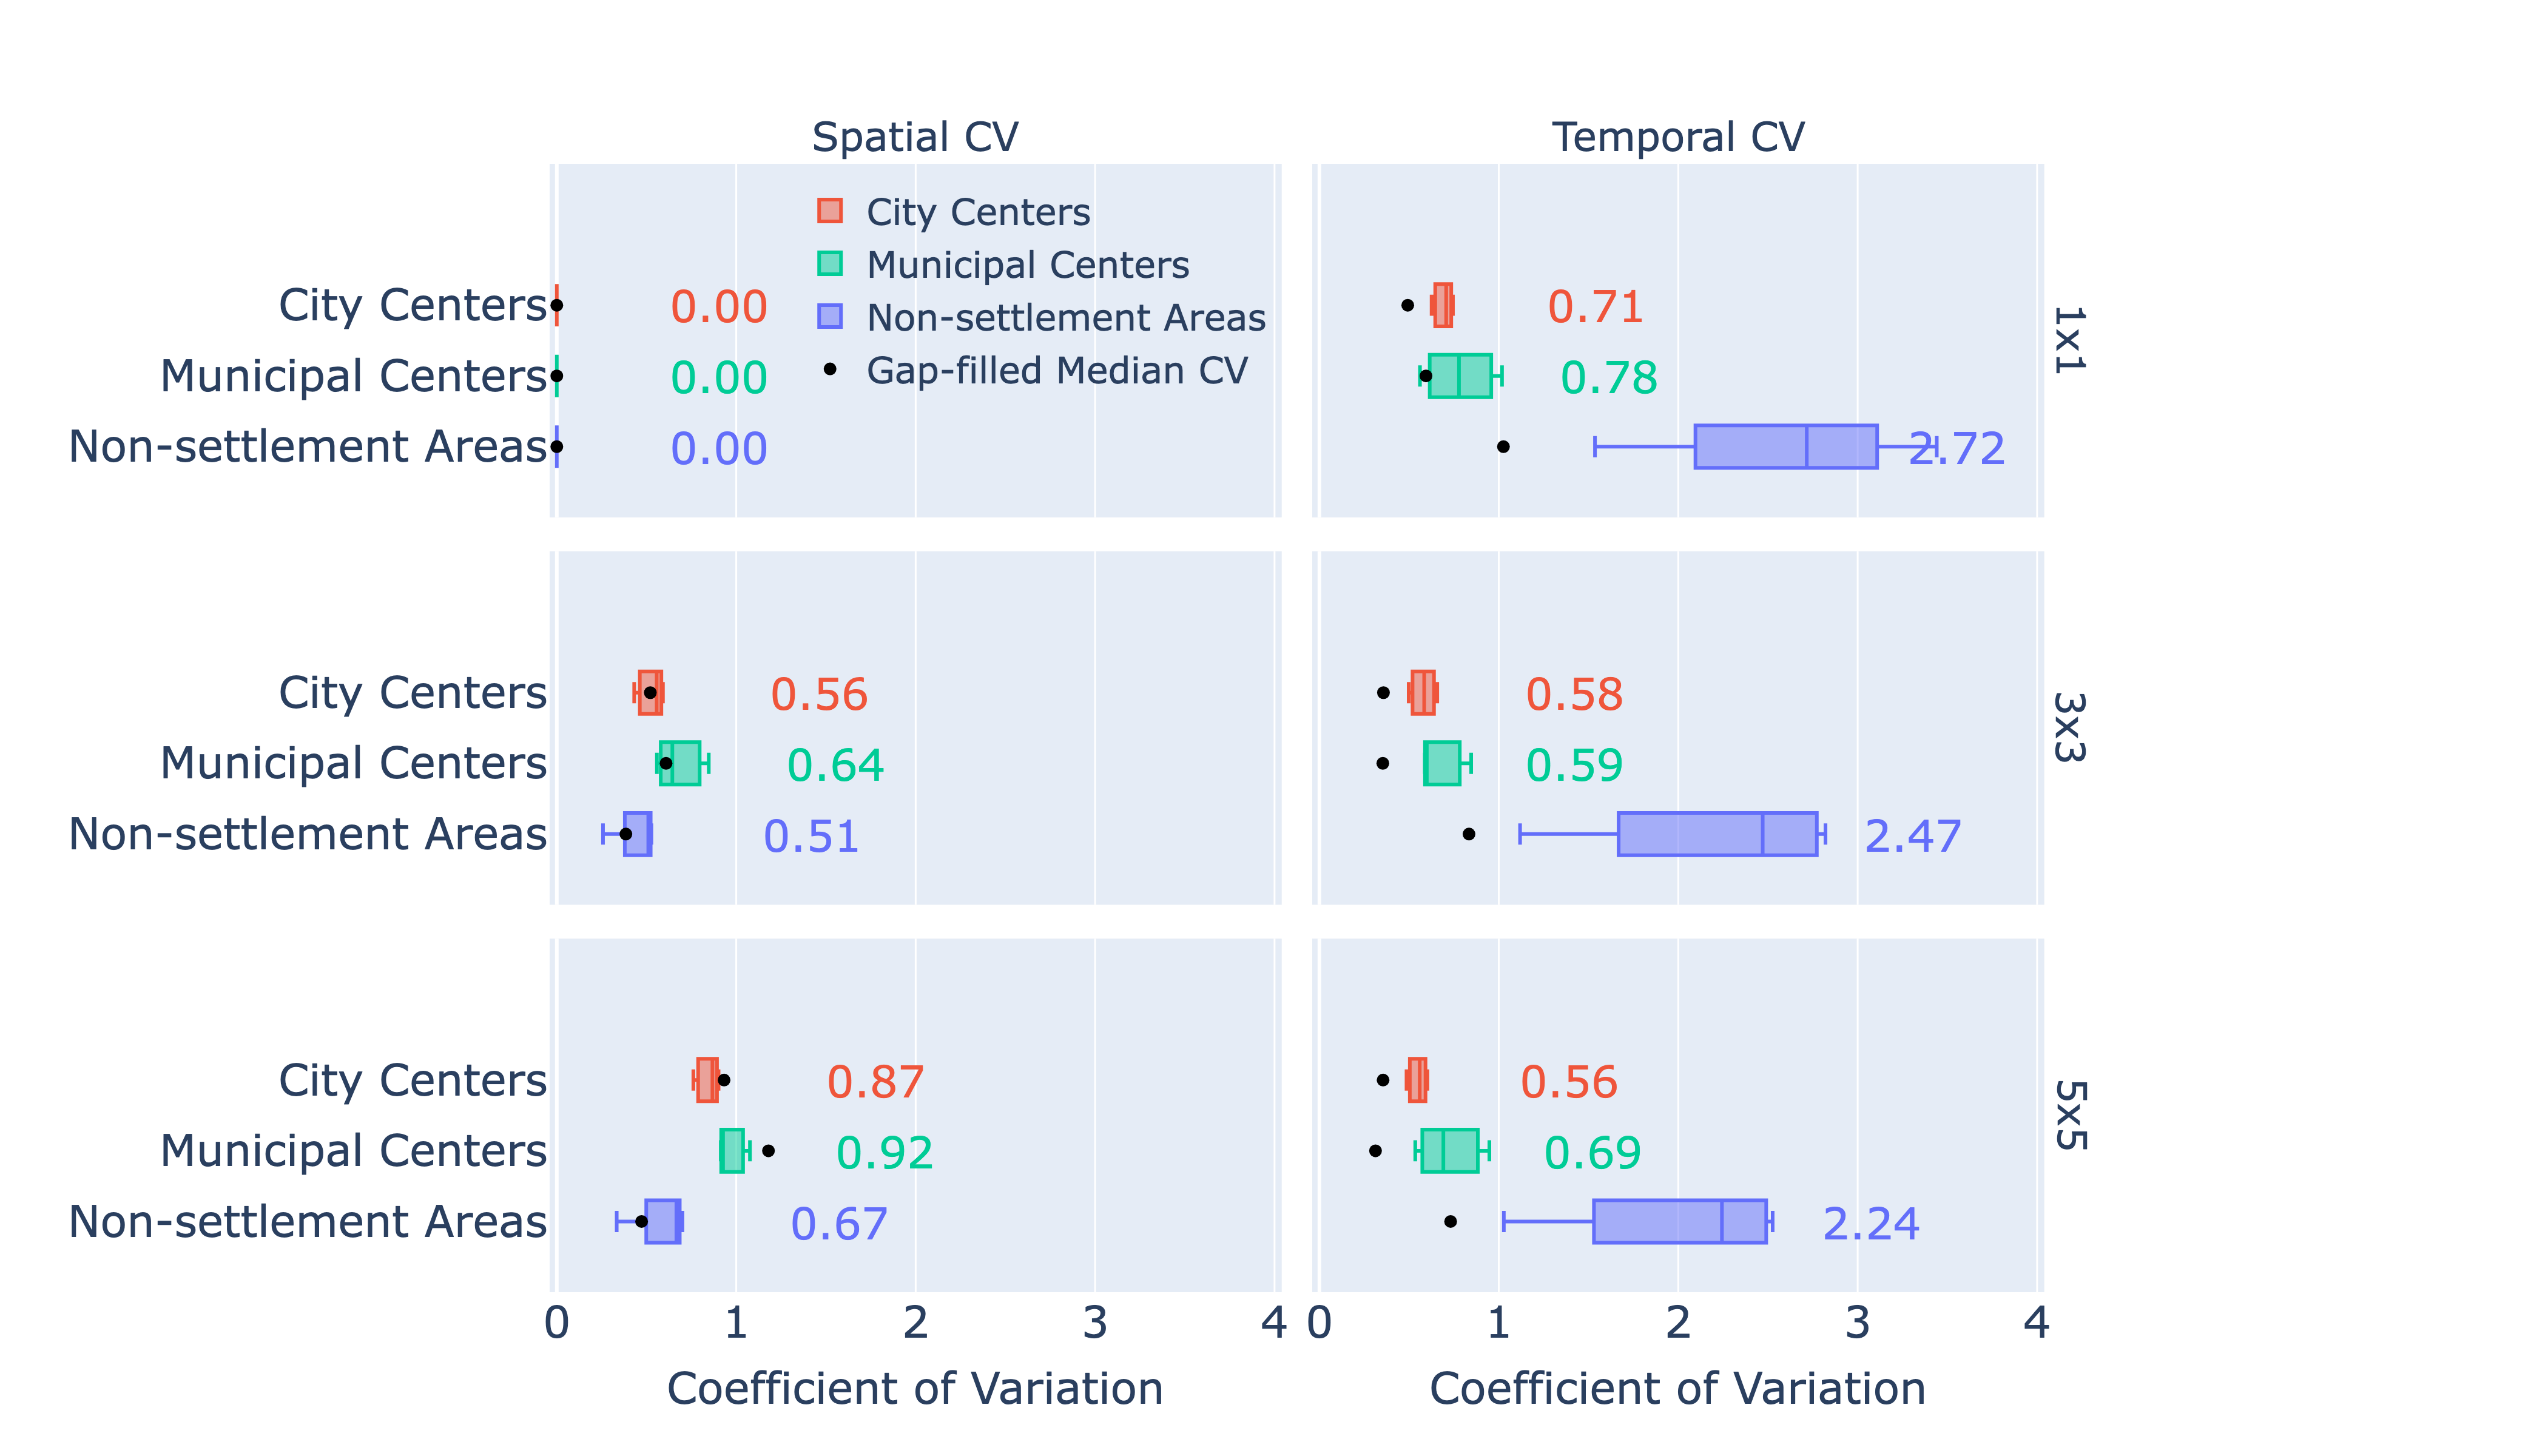
\includegraphics[
            width=0.95\linewidth,
            keepaspectratio
        ]{figs/fig_04_poi_cv_by_kernel_and_settlement_2013.png}
        \caption{Spatial CV (left) and temporal CV (right) of DNB-BRDF radiance across POI groups during 2013. Rows represent the three kernel supports. Box plots show the distribution of POI-level CV values, and coloured annotations report group medians. Black points mark the corresponding median CV of gap-filled radiance.}
        \label{fig:poi_cv}
    \end{figure}
    
    \subsection{Local-Scale Observability and Stability}
        
        Table~\ref{tab:poi_summary} summarises spatial completeness, temporal completeness, and maximum consecutive dropout duration for the ten POIs listed in Supplementary Table~S1. Across city and municipal centres, $TC_{50}$ ranges from 28.9\% to 33.5\%, indicating admissible observations on approximately one-third of calendar days. Increasing kernel support generally reduces mean SC, while changes in TC are smaller. Between $1\times1$ and $5\times5$, city-centre SC decreases from 31.1\% to 26.5\%, compared with a decline in TC from 31.1\% to 28.9\%.
        
        Maximum consecutive dropout duration varies more strongly among individual POIs than the grouped completeness values suggest. Individual maxima range from 20 to 39 days (Supplementary Table~S2). The maximum remains unchanged across supports for nine POIs. Tacloban City Centre is the exception: its maximum dropout increases from 21 days at $1\times1$ and $3\times3$ to 38 days at $5\times5$, while TC decreases from 32.6\% to 29.9\% between the smallest and largest supports. Supplementary Figure~S5 shows the placement of these intervals alongside daily SC and radiance.
        
        Radiance stability diagnostics (Figure~\ref{fig:poi_cv}) show systematic differences by settlement context and kernel support. Temporal CV is lowest in city centres, intermediate in municipal centres, and highest in non-settlement locations, where median values exceed 2 across all supports. Increasing support from $1\times1$ to $5\times5$ reduces median temporal CV from 0.71 to 0.56 in city centres and from 2.72 to 2.24 in non-settlement areas. Spatial CV is zero at $1\times1$ and increases at the broader supports. At $5\times5$, municipal centres have the highest median spatial CV of 0.92, followed by city centres at 0.87 and non-settlement areas at 0.67.
        
        A consistent product-level contrast is also evident in Figure~\ref{fig:poi_cv}: gap-filled radiance has lower median temporal CV than DNB-BRDF across all POI groups and kernel supports. Regional and single-pixel comparisons in Supplementary Figures~S1--S2 show smoother gap-filled trajectories during periods of sparse direct observations, while Figure~S5 extends the comparison across all ten POIs. The 2013 pre--post Haiyan mean radiance contrast also changes with spatial support. For city centres, the contrast decreases in magnitude from approximately $-15$ to $-7\,\mathrm{nW\,cm^{-2}\,sr^{-1}}$ between $1\times1$ and $5\times5$ (Supplementary Figure~S4).
    
    \subsection{Settlement-Scale Observability Diagnostics}
    
    \begin{table}[!t]
        \centering
        \caption{Settlement-scale observability diagnostics for Samar--Leyte during 2013, grouped from the individual GHSL classes in Table~\ref{tab:smod}. SC, TC, and CV are unweighted arithmetic means of constituent-class values; pixel shares are summed. Maximum dropout duration is the longest constituent-class run at $\tau=0.5$. TC columns identify the SC threshold applied.}
        \label{tab:settlement_grouped}
    
        \footnotesize
        \setlength{\tabcolsep}{4pt}
        \renewcommand{\arraystretch}{1.15}
    
        \resizebox{\linewidth}{!}{%
        \begin{tabular}{lcccccccc}
            \toprule
    
            \textbf{Settlement Group} &
            \textbf{Pixel Share} &
            \multicolumn{5}{c}{\textbf{Observational Completeness}} &
            \multicolumn{2}{c}{\textbf{Radiance Variability}} \\
    
            \cmidrule(lr){3-7}
            \cmidrule(lr){8-9}
    
            &
            \textbf{(\%)} &
            \textbf{SC, \%} &
            \multicolumn{3}{c}{\textbf{TC, \%}} &
            \textbf{Max Dropout} &
            \textbf{Temporal CV} &
            \textbf{Spatial CV} \\
    
            \cmidrule(lr){4-6}
    
            &
            &
            &
            $\tau=25\%$ &
            $\tau=50\%$ &
            $\tau=75\%$ &
            \textbf{(days)} &
            &
            \\
    
            \midrule
    
            Urban Centre
            & 0.47
            & 37.3
            & 43.8
            & 34.8
            & 25.8
            & 22
            & 0.71
            & 1.39 \\
    
            Urban Cluster
            & 11.78
            & 45.8
            & 49.5
            & 39.2
            & 30.4
            & 22
            & 0.66
            & 1.44 \\
    
            Non-urban Cells
            & 86.70
            & 32.0
            & 47.9
            & 33.5
            & 15.5
            & 23
            & 0.68
            & 1.25 \\
    
            Water
            & 1.05
            & 54.0
            & 52.9
            & 41.9
            & 30.1
            & 20
            & 1.47
            & 1.14 \\
    
            \bottomrule
        \end{tabular}%
        }
    \end{table}
    
    \begin{figure*}[!b]
        \centering
        \includegraphics[width=\linewidth]{figs/fig_05_global_temporal_completeness.png}
        \caption{Per-pixel temporal completeness of daily VIIRS Black Marble DNB-BRDF observations during 2013, with the Philippines shown in detail. Values represent the percentage of evaluated days with a valid DNB-BRDF retrieval at each pixel. White areas denote missing completeness values. VNP46A2 data were processed in Google Earth Engine; inset basemap \textcopyright{} OpenStreetMap contributors.}
        \label{fig:temporal_maps}
    \end{figure*}
    
        Table~\ref{tab:settlement_grouped} reports settlement-scale observability diagnostics for Samar--Leyte using GHSL SMOD classes. Among the land-based groups, mean SC ranges from 32.0\% in non-urban cells to 45.8\% in urban clusters. Temporal completeness decreases as the spatial validity requirement becomes stricter, but the response differs between groups. Urban clusters and non-urban cells have similar TC at $\tau=25\%$, at 49.5\% and 47.9\%, respectively. At $\tau=75\%$, their values separate to 30.4\% and 15.5\%. The corresponding declines are 19.1 and 32.4 percentage points.
        
        At $\tau=50\%$, maximum dropout durations occupy a narrower range than the completeness metrics. Group maxima are 22 days for urban centres and urban clusters, 23 days for non-urban cells, and 20 days for water. Individual-class maxima range from 20 to 23 days (Supplementary Table~S3). The class-level series in Supplementary Figure~S6 show these gaps alongside contrasting radiance levels, with stronger urban signals and low-intensity rural and water backgrounds.
        
        Individual classes also show a larger range in spatial CV than temporal CV. Spatial CV ranges from 0.89 in very low-density rural cells to 1.76 in dense urban clusters, whereas land-based temporal CV ranges from 0.63 to 0.76 (Supplementary Table~S3).
        
        Settlement composition is strongly imbalanced across Samar--Leyte. Urban centres account for 0.47\% of analysed pixels and urban clusters for 11.78\%, while non-urban cells account for 86.70\%. Supplementary Figure~S7 illustrates the compact urban footprints and additional settlement areas incorporated by the cumulative thematic masks derived from these classes.
        
        The global TC map in Figure~\ref{fig:temporal_maps} places the Samar--Leyte results within a wider geographical pattern. Annual completeness is generally higher across many arid and temperate regions and lower across equatorial and monsoonal regions. The Philippines forms part of a coherent low-completeness belt across maritime Southeast Asia. Long-term Samar--Leyte diagnostics in Supplementary Figure~S3 show recurring low-SC intervals throughout 2012--2024, with pronounced seasonal and interannual variation.
        
    \subsection{Reliability-Qualified Alignment Between Stratified NTL and Sub-Grid Load}
    
        Figure~\ref{fig:threshold_sweep} summarises the systematic sweep of spatial completeness thresholds across cumulative GHSL thematic masks in Samar--Leyte at $W=1$. The component heatmaps show how Pearson correlation and retained direct-date coverage vary jointly across configurations, while the composite score identifies the highest-ranked mask--threshold combination.
        
    \begin{figure*}[!t]
        \centering
        \subfigure[Pearson correlation, $r$.]{%
            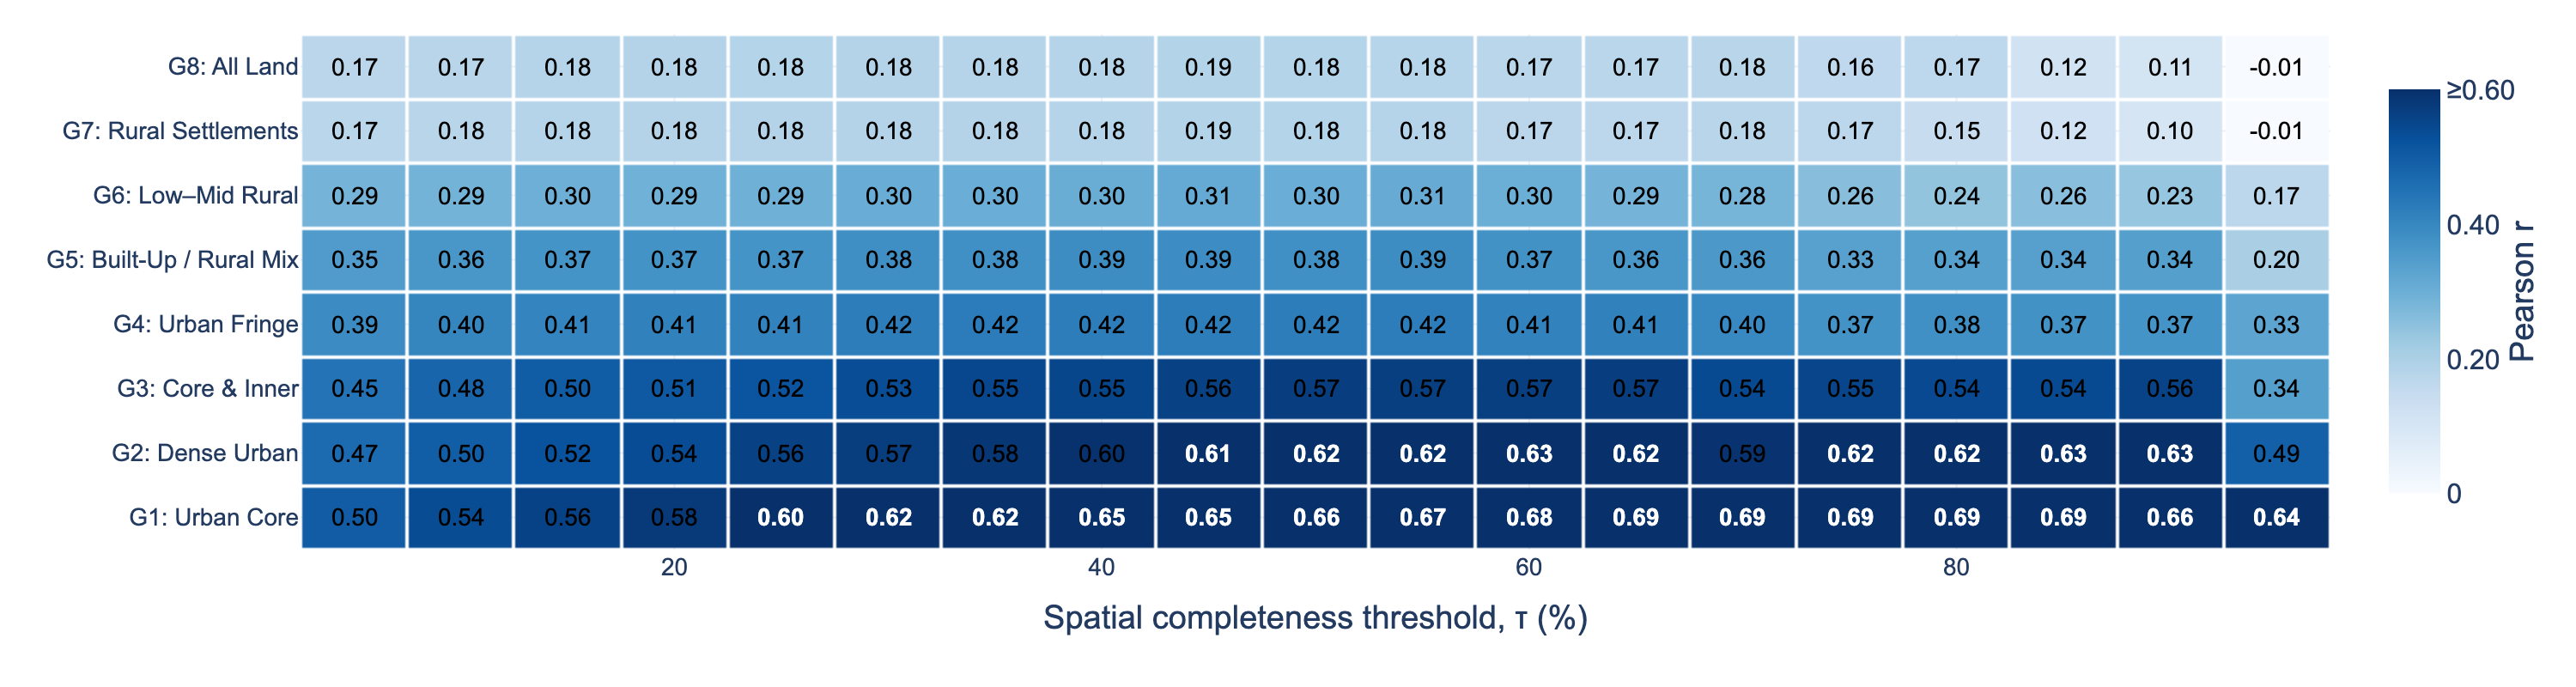
\includegraphics[width=\linewidth]
            {figs/fig_06a_native_daily_r.png}
            \label{fig:daily_r}
        }
    
        \par\medskip
    
        \subfigure[Retained direct-date coverage, $N_{\%}$.]{%
            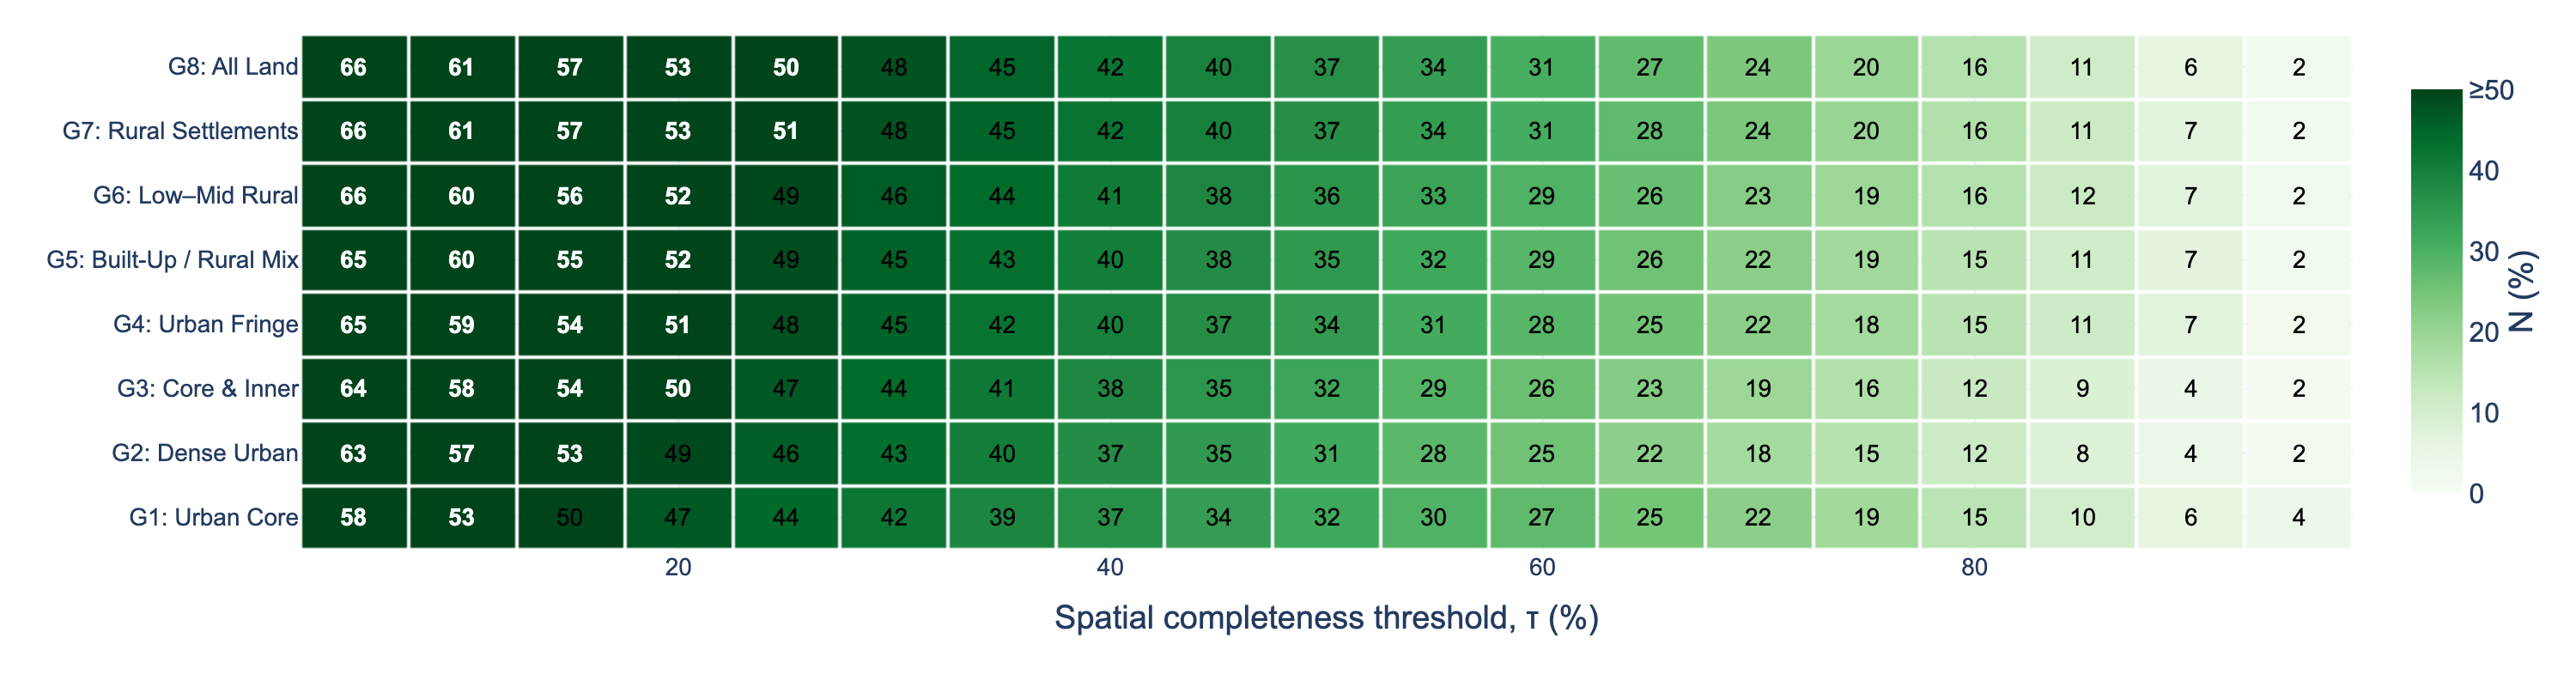
\includegraphics[width=\linewidth]
            {figs/fig_06b_native_daily_N.png}
            \label{fig:daily_N}
        }
    
        \par\medskip
    
        \subfigure[Composite score, $S_{\mathrm{daily}}$.]{%
            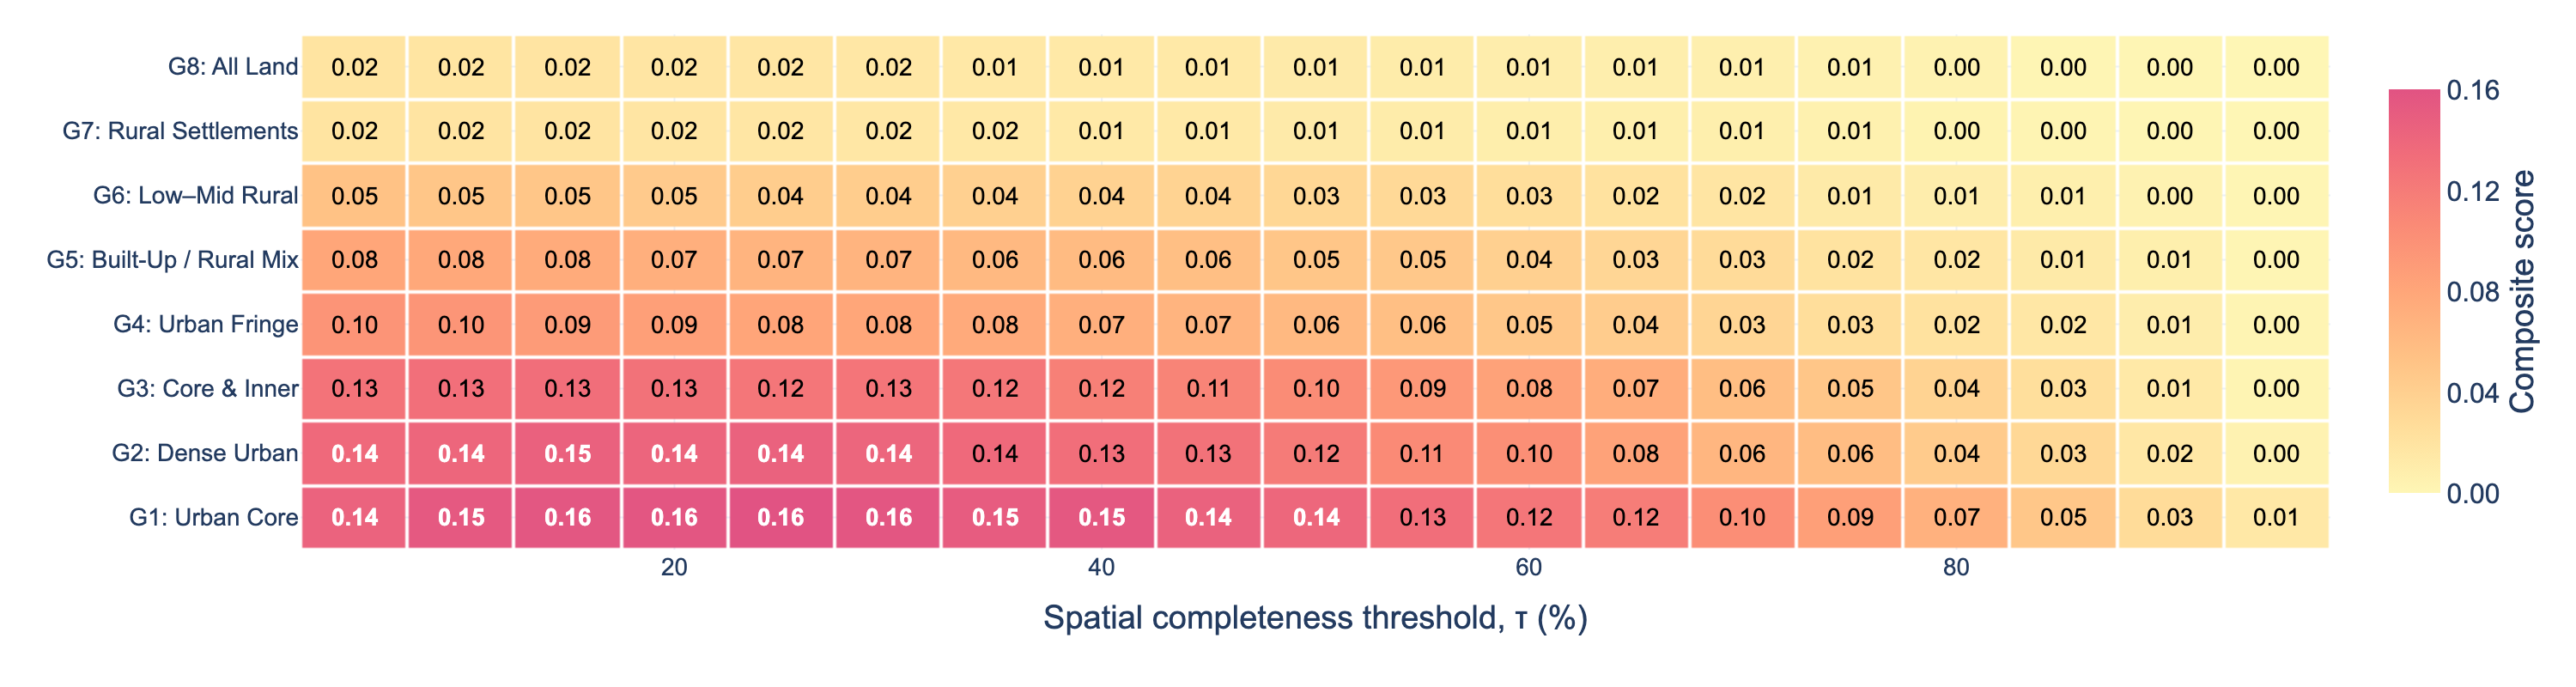
\includegraphics[width=\linewidth]
            {figs/fig_06c_native_daily_score.png}
            \label{fig:daily_score}
        }
    
        \caption{Systematic sweep of SC thresholds ($\tau$) across cumulative GHSL masks G1--G8 in Samar--Leyte at $W=1$. Cell values report Pearson $r$, retained direct-date coverage $N_{\%}$, and composite score $S_{\mathrm{daily}}$. Correlation and coverage colour scales saturate at 0.60 and 50\%, respectively; the score scale extends to its observed maximum. Bold annotations identify $r\geq0.60$, $N_{\%}\geq50\%$, and scores at or above the 90th percentile in panels (a), (b), and (c), respectively.}
        \label{fig:threshold_sweep}
    \end{figure*}
    
        Alignment varies with both thematic support and SC threshold. Urban-focused masks generally show stronger correspondence with NGCP load than the broadest masks, while retained direct-date coverage declines as $\tau$ increases. For G1 Urban Core, increasing $\tau$ from 25\% to 40\% raises $r$ from 0.602 to 0.650 and reduces coverage from 44.2\% to 36.6\%. Over the same interval, the composite score decreases from 0.1600 to 0.1546. G1 at $\tau=25\%$ achieves the highest score in the Samar--Leyte sweep.
        
        Sensitivity to the scoring rule changes the highest-ranked configuration in four of the five sub-grids (Supplementary Figure~S11). Both mask and threshold change in Samar--Leyte, Bohol, and Negros; Cebu retains G1 but shifts its threshold, while Panay retains the same mask and threshold. In Samar--Leyte, the linear rule selects G2 at $\tau=5\%$, with $r=0.466$ and coverage of 63.2\%, compared with G1 at $\tau=25\%$, $r=0.602$, and coverage of 44.2\% under the squared rule. Agreement between complete rankings also varies: Spearman's $\rho$ is approximately 0.95 in Samar--Leyte and 0.37 in Cebu.
    
    \begin{figure*}[p]
        \centering
        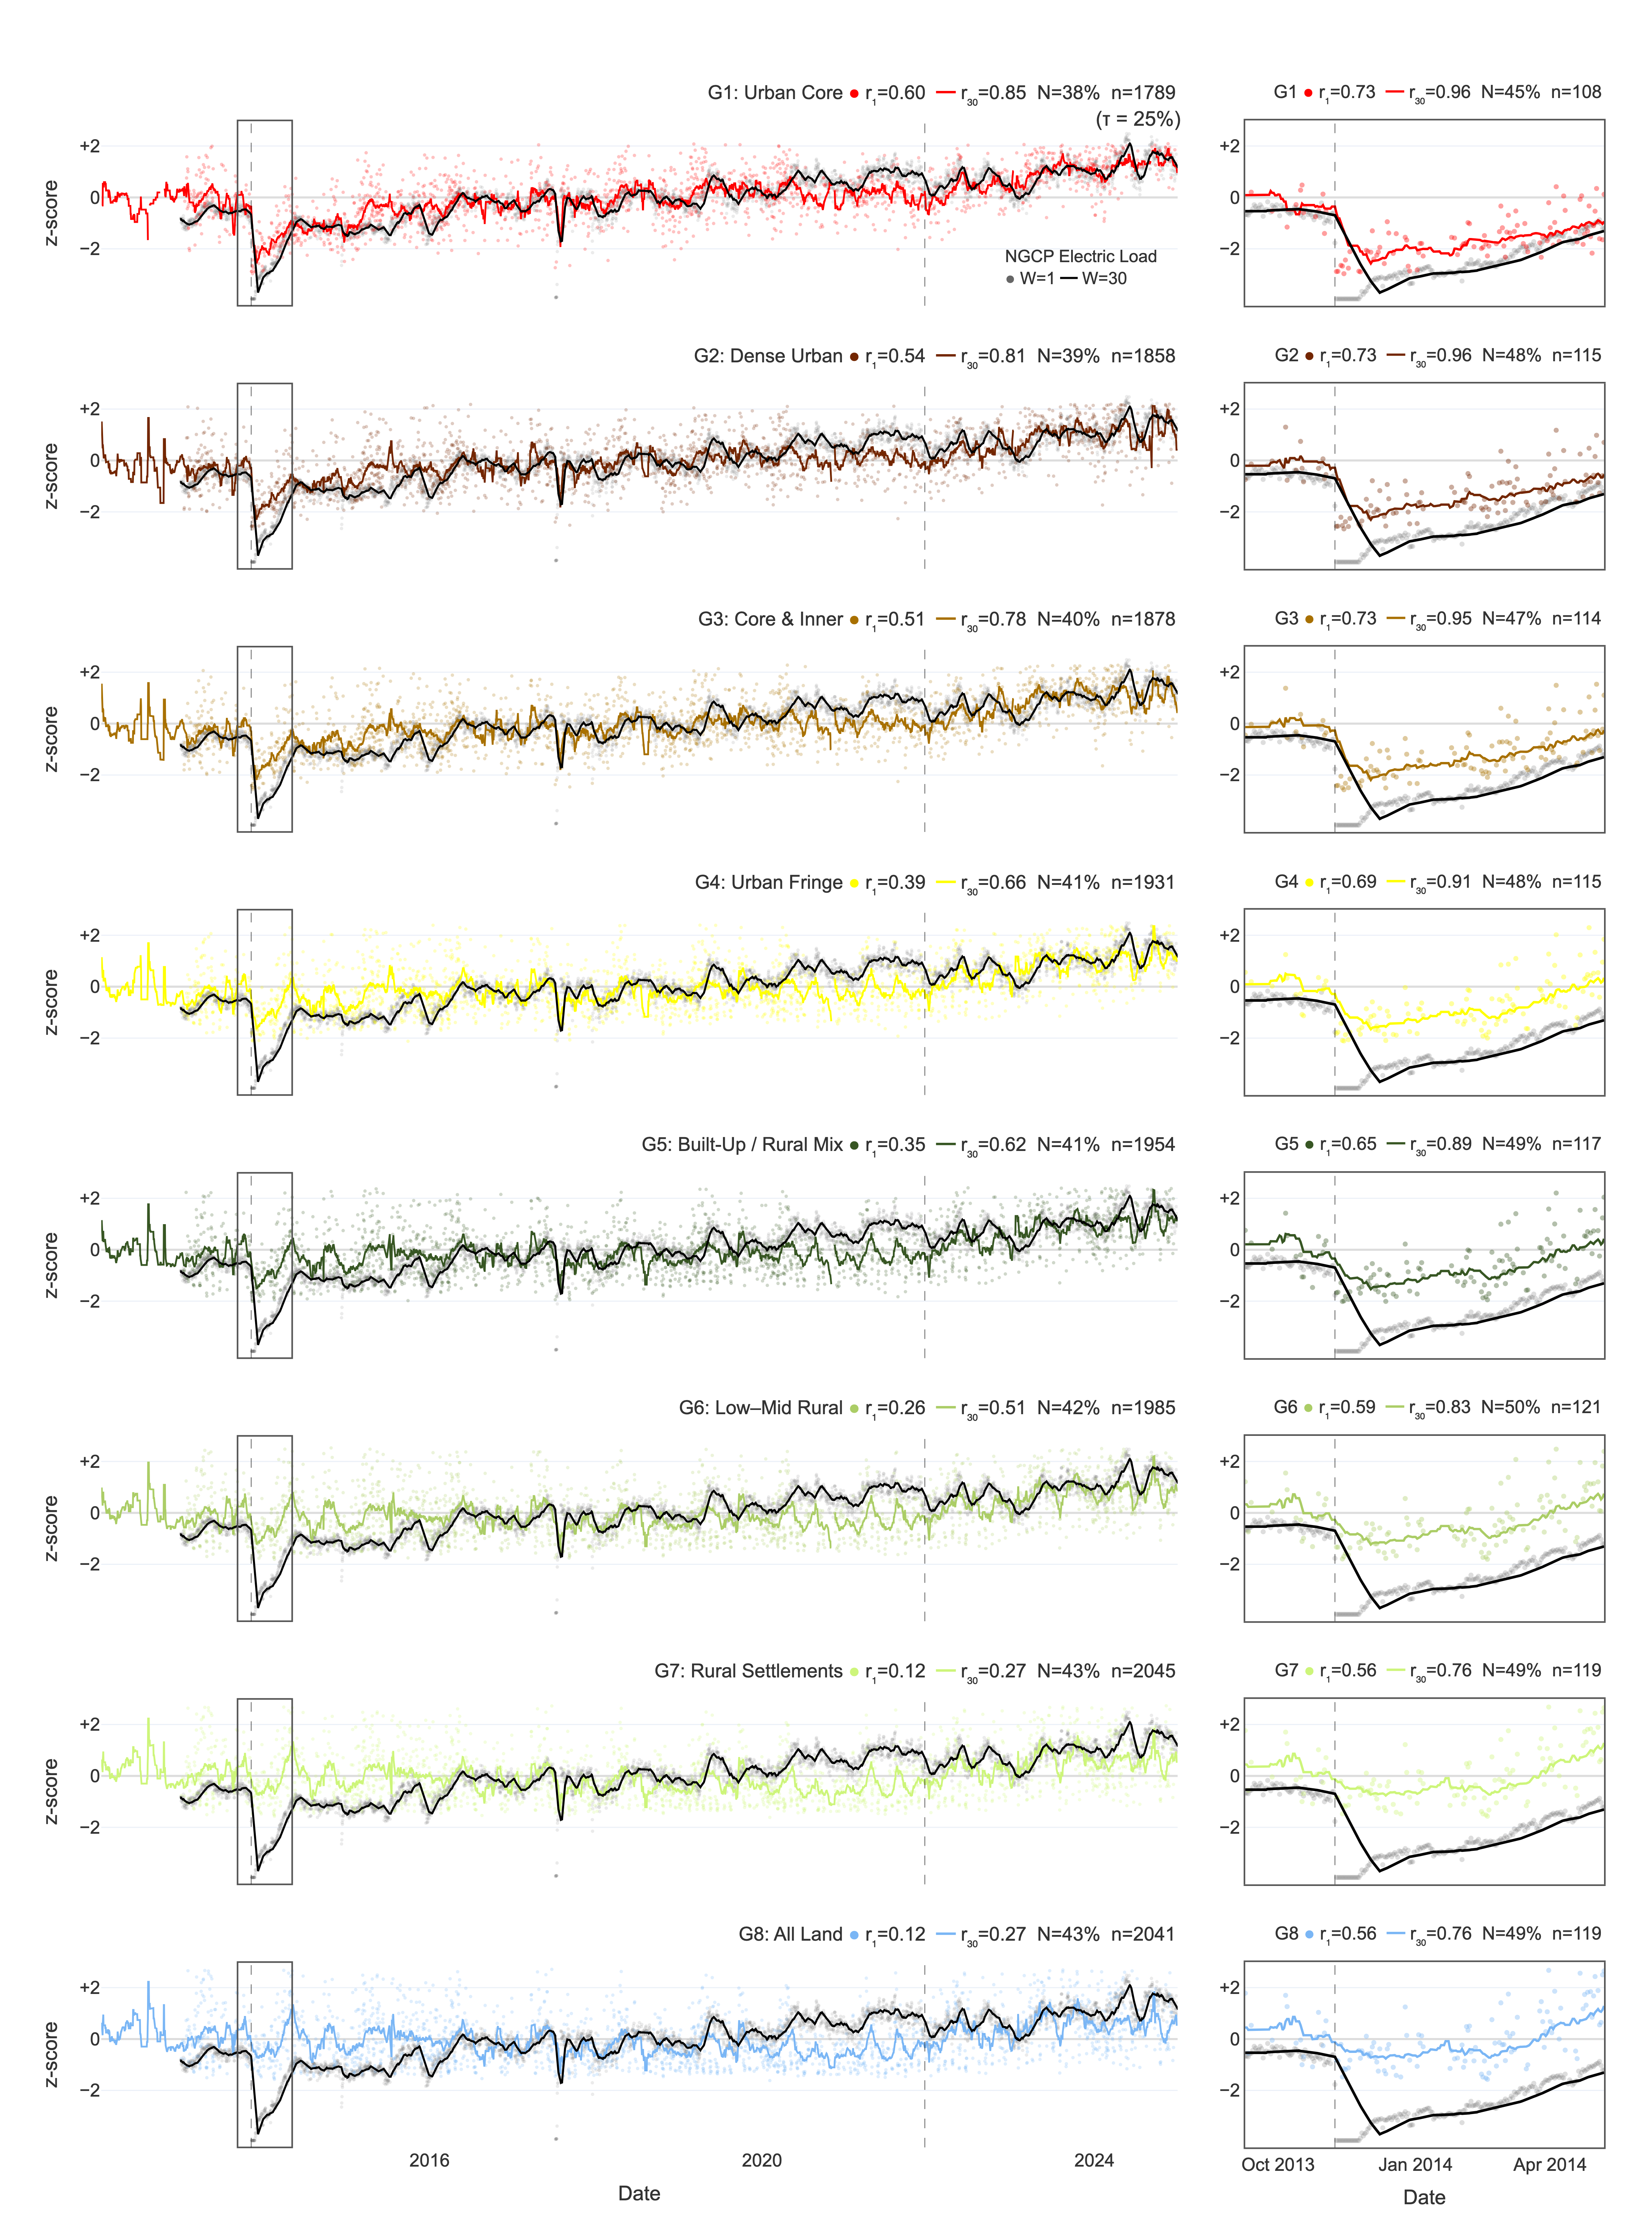
\includegraphics[width=\linewidth,keepaspectratio]{figs/fig_07_samar_leyte.png}
        \caption{GHSL-stratified NTL--NGCP alignment for Samar--Leyte at $\tau=25\%$, with masks G1--G8 arranged from top to bottom. Coloured and grey points represent NTL and NGCP observations at $W=1$, respectively; coloured and black lines show 30-day trailing means ($W=30$). Left panels show the full record, with boxes marking the intervals enlarged on the right, from 60 days before to 180 days after Haiyan landfall on 8 November 2013. Zooms retain the full-record z-score normalisation. Annotations report $r_1$ on directly paired dates, $r_{30}$ on dates with paired trailing estimates, and the number ($n$) and percentage ($N_{\%}$) of calendar days with directly paired observations in each panel period.}
        \label{fig:alignment_25pct}
    \end{figure*}
    
        Figure~\ref{fig:alignment_25pct} presents the Samar--Leyte time series for all eight masks at the threshold selected for G1. In the full-record panels, $r_1$ decreases from 0.60 for G1 to 0.12 for G8, although G8 retains a larger share of directly paired calendar days. The Haiyan zooms show a marked decline in NGCP load followed by a gradual rise, with urban-focused radiance following this broader trajectory more closely than the broadest masks. Differences between masks are smaller within the event window, where $r_1$ is 0.73 for G1 and 0.56 for G8.
        
        The threshold-specific comparisons in Supplementary Figures~S8--S9 extend this fixed-threshold view. Urban-focused $W=30$ series retain the broad full-record trajectory across $\tau=25$--75\%, while local fluctuations and the continuity of the estimates vary between thresholds. The Haiyan enlargements show corresponding differences in the profiles around landfall and the subsequent rise.
    
    \subsection{Regional Assessment of Reliability-Qualified Configurations}
    
        Figure~\ref{fig:regional_daily_heatmaps} extends the $W=1$ sweep to Bohol, Cebu, Negros, and Panay. The red outlines locate each selected configuration on the corresponding correlation, coverage, and score surfaces. Table~\ref{tab:transferability} reports the selected settings across all five sub-grids, including Samar--Leyte.
        
    \begin{figure*}[!t]
        \centering
        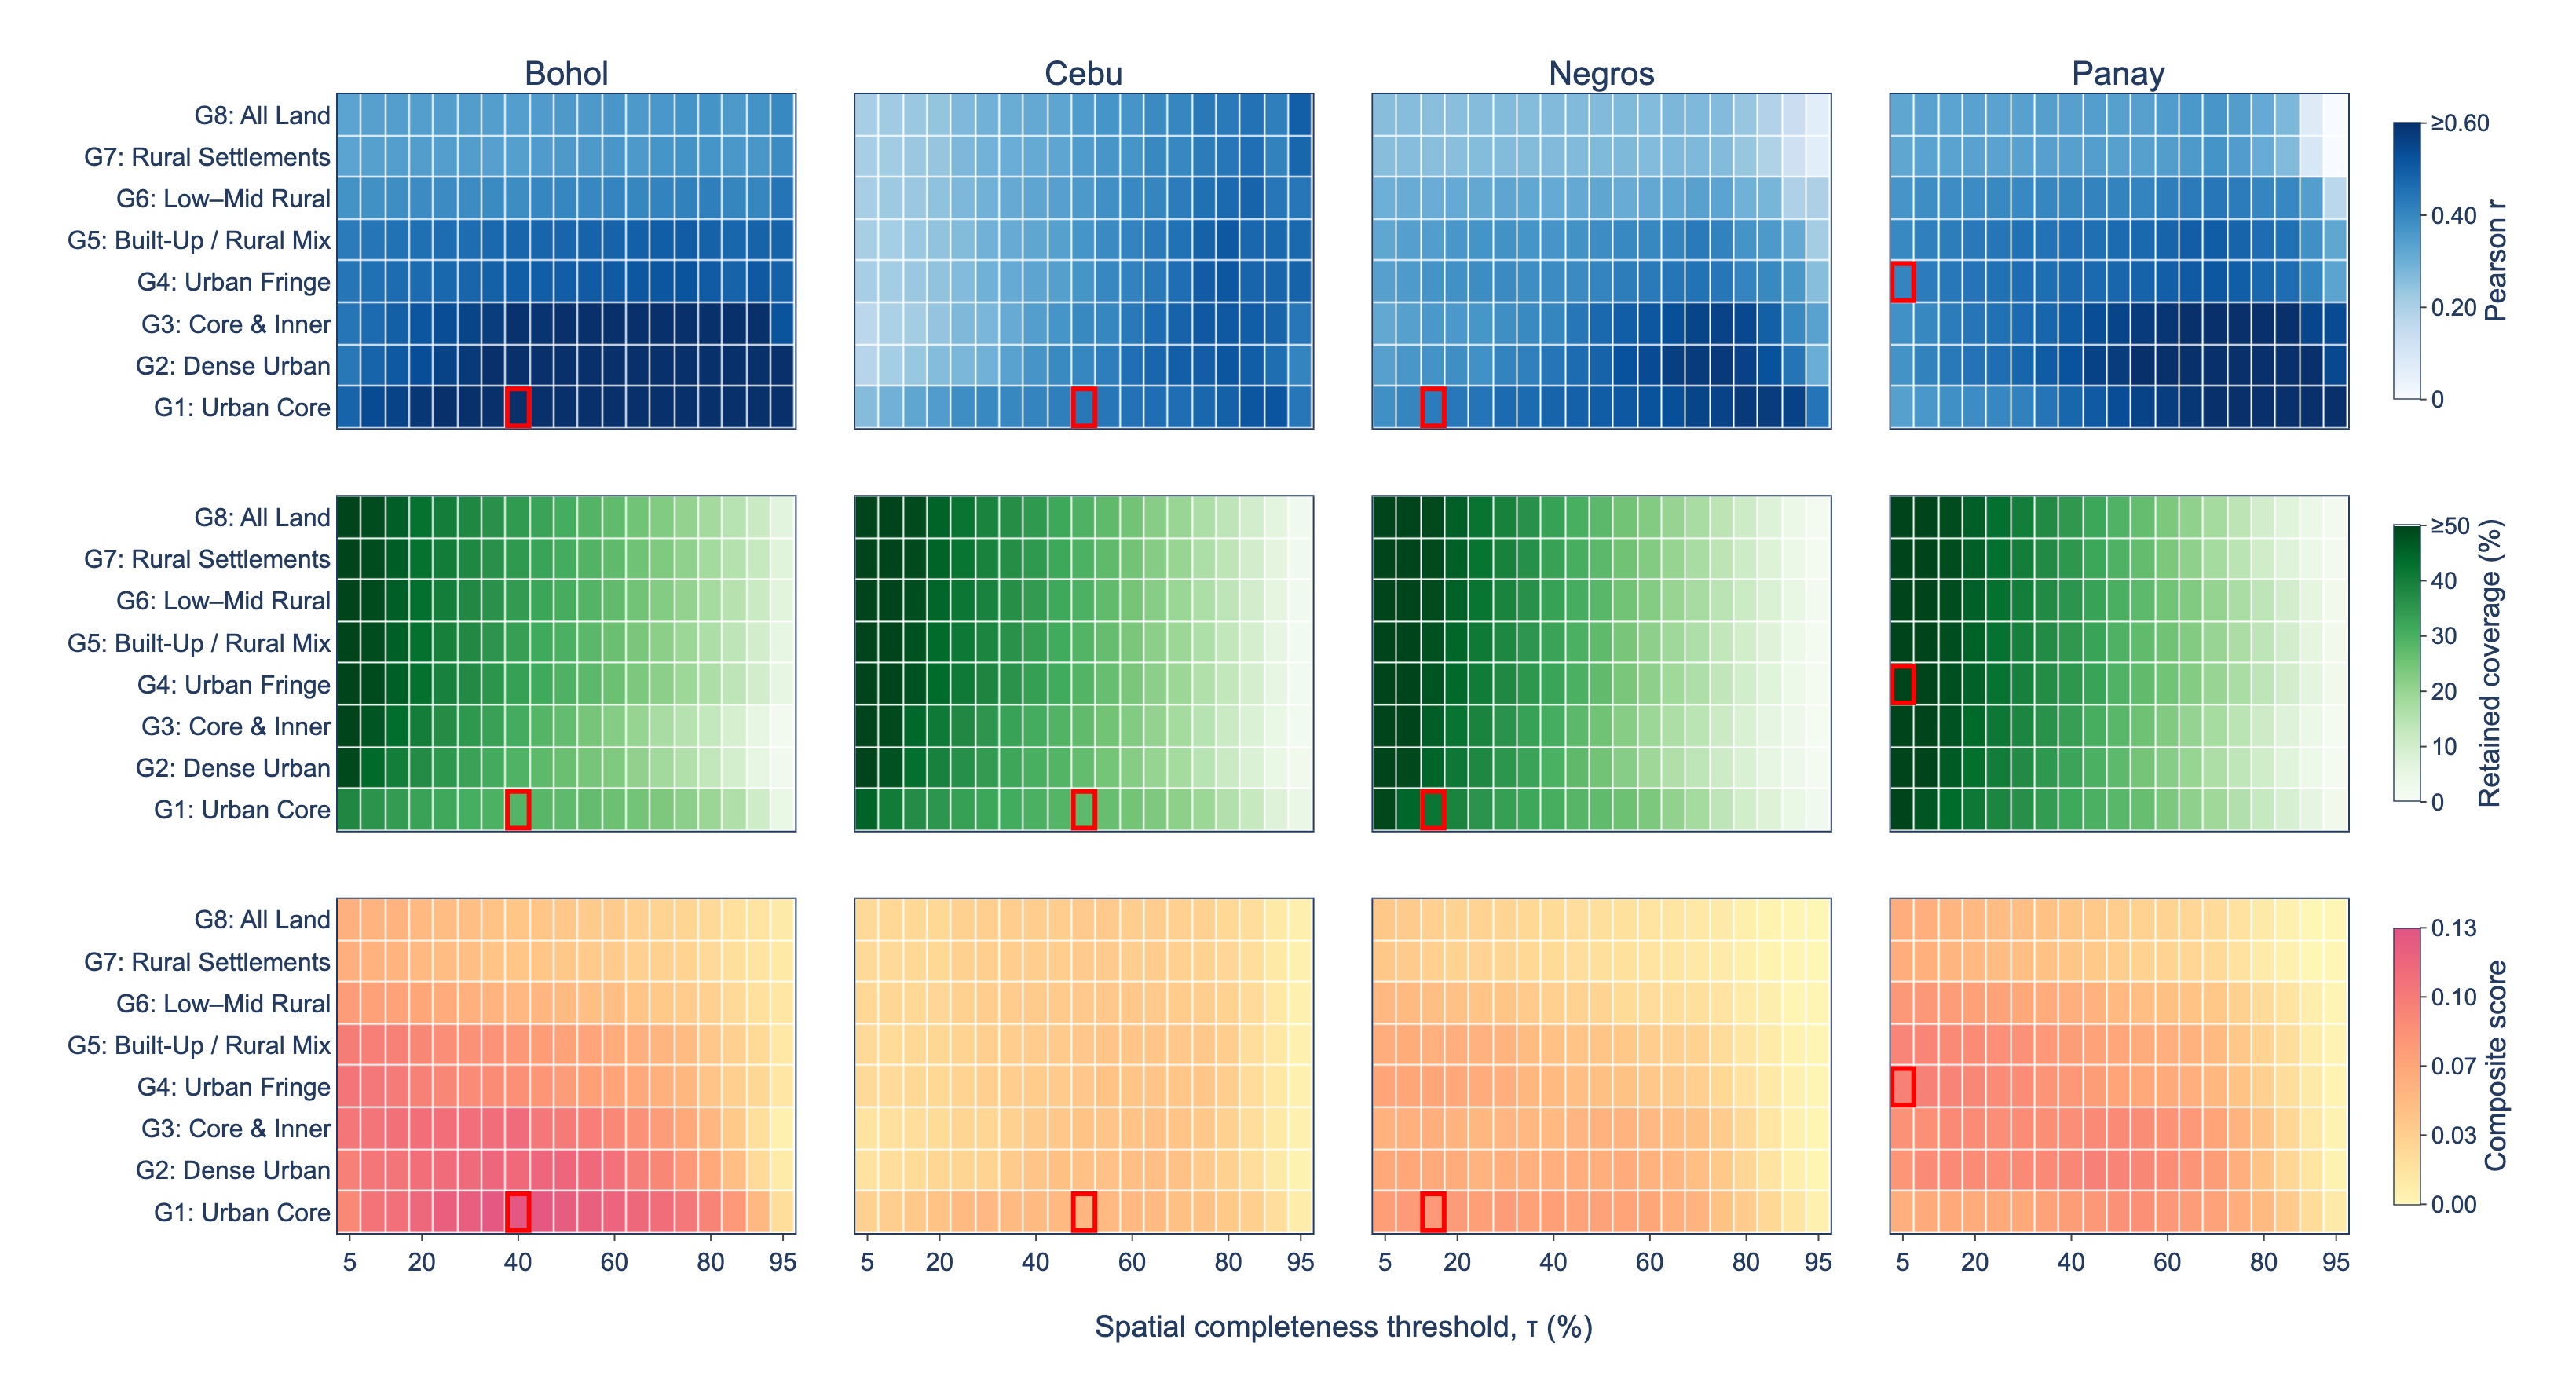
\includegraphics[width=\linewidth]{figs/fig_08_regional_daily_heatmaps.png}
        \caption{Configuration sweeps at $W=1$ for Bohol, Cebu, Negros, and Panay. From top to bottom, rows show Pearson $r$, retained direct-date coverage $N_{\%}$, and composite score $S_{\mathrm{daily}}$ across cumulative GHSL masks and SC thresholds. Correlation and coverage colour scales match Figure~\ref{fig:threshold_sweep}. Red outlines mark the highest-scoring configuration in each sub-grid at the same mask and threshold in all three rows. These settings are used for the time series in Figure~\ref{fig:visayas_timeseries}.}
        \label{fig:regional_daily_heatmaps}
    \end{figure*}
    
    \begin{table}[!t]
        \centering
        \caption{Highest-scoring NTL--load configurations at $W=1$ for the five Visayas sub-grids. Configurations maximise $S_{\mathrm{daily}}$ within each sub-grid. Retained direct-date coverage ($N_{\%}$) is the percentage of available NGCP load dates with a qualifying NTL observation, and $n$ is the number of paired days.}
        \label{tab:transferability}
        \footnotesize
        \setlength{\tabcolsep}{4pt}
        \begin{tabular}{llrrrrr}
            \toprule
            Sub-grid & GHSL mask & $\tau$ (\%) & $S_{\mathrm{daily}}$ & $r$ & $N_{\%}$ & $n$ \\
            \midrule
            Samar--Leyte & G1 Urban Core   & 25 & 0.1600 & 0.602 & 44.2 & 1936 \\
            Bohol        & G1 Urban Core   & 40 & 0.1267 & 0.660 & 29.1 & 1275 \\
            Cebu         & G1 Urban Core   & 50 & 0.0525 & 0.435 & 27.7 & 1216 \\
            Negros       & G1 Urban Core   & 15 & 0.0753 & 0.424 & 41.8 & 1834 \\
            Panay        & G4 Urban Fringe &  5 & 0.0940 & 0.406 & 56.9 & 2495 \\
            \bottomrule
        \end{tabular}
    \end{table}
    
        G1 Urban Core is selected in Samar--Leyte, Bohol, Cebu, and Negros, while G4 Urban Fringe is selected in Panay. The selected thresholds range from 5\% in Panay to 50\% in Cebu. Among the selected configurations, Bohol has the highest correlation of 0.660, while Panay retains the greatest direct-date coverage of 56.9\%. G1 also occupies all five highest-ranked positions within each of the first four sub-grids; Panay's leading configurations include both G4 and G2 (Supplementary Table~S4).
        
        The correlation--coverage trajectories in Supplementary Figure~S10 show how nearby scores can correspond to different combinations of association and retention. In Panay, G4 at $\tau=5\%$ scores 0.0940, compared with 0.0937 for G2 at $\tau=45\%$. Their correlations are 0.406 and 0.559, respectively, while retained coverage differs by 26.9 percentage points, at 56.9\% and 30.0\%.
    
    \begin{figure*}[!b]
        \centering
        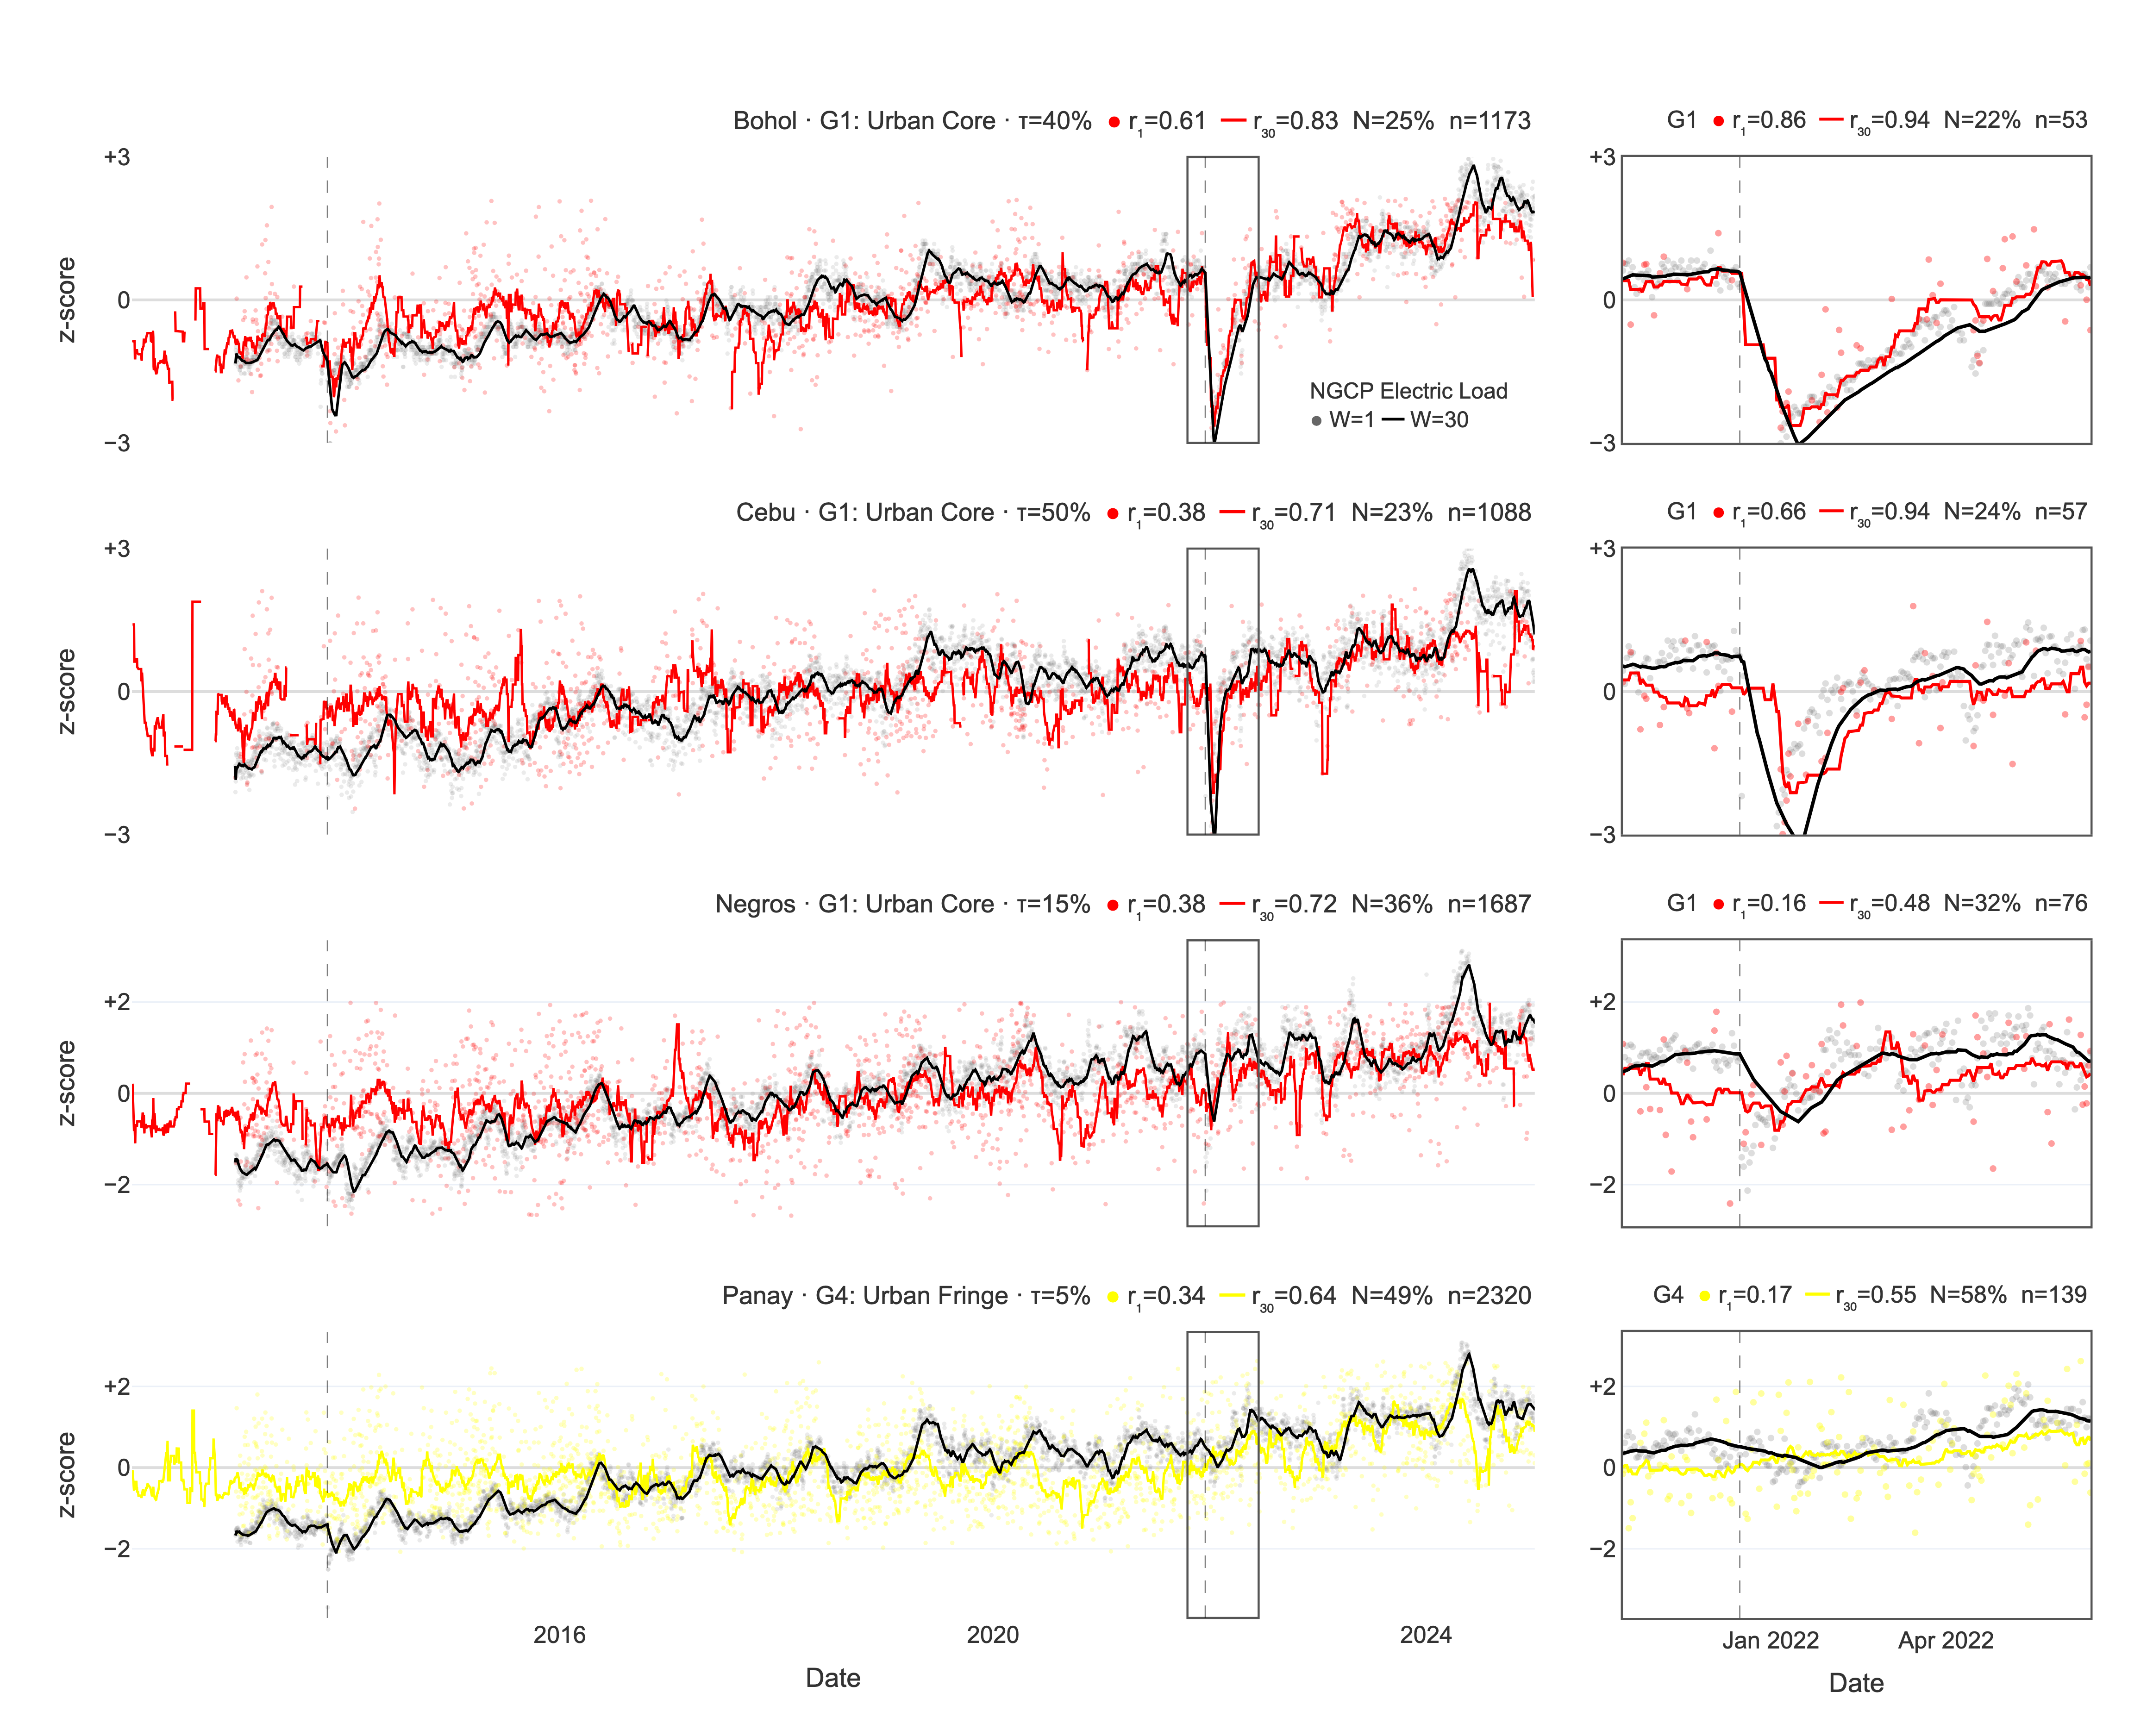
\includegraphics[width=\linewidth]{figs/fig_08_selected_regions_rai.png}
        \caption{Regional NTL--NGCP alignment for Bohol (G1, $\tau=40\%$), Cebu (G1, $\tau=50\%$), Negros (G1, $\tau=15\%$), and Panay (G4, $\tau=5\%$), from top to bottom. Coloured and grey points represent NTL and NGCP observations at $W=1$, respectively; coloured and black lines show 30-day trailing means ($W=30$). Left panels show the full record, with boxes marking the intervals enlarged on the right, from 60 days before to 180 days after Rai landfall on 16 December 2021. Zooms retain the full-record z-score normalisation. Panel annotations report $r_1$ and $r_{30}$ on directly paired observation dates, together with the number ($n$) and percentage ($N_{\%}$) of calendar days with directly paired observations in each panel period.}
        \label{fig:visayas_timeseries}
    \end{figure*}

    \begin{figure*}[!t]
        \centering
        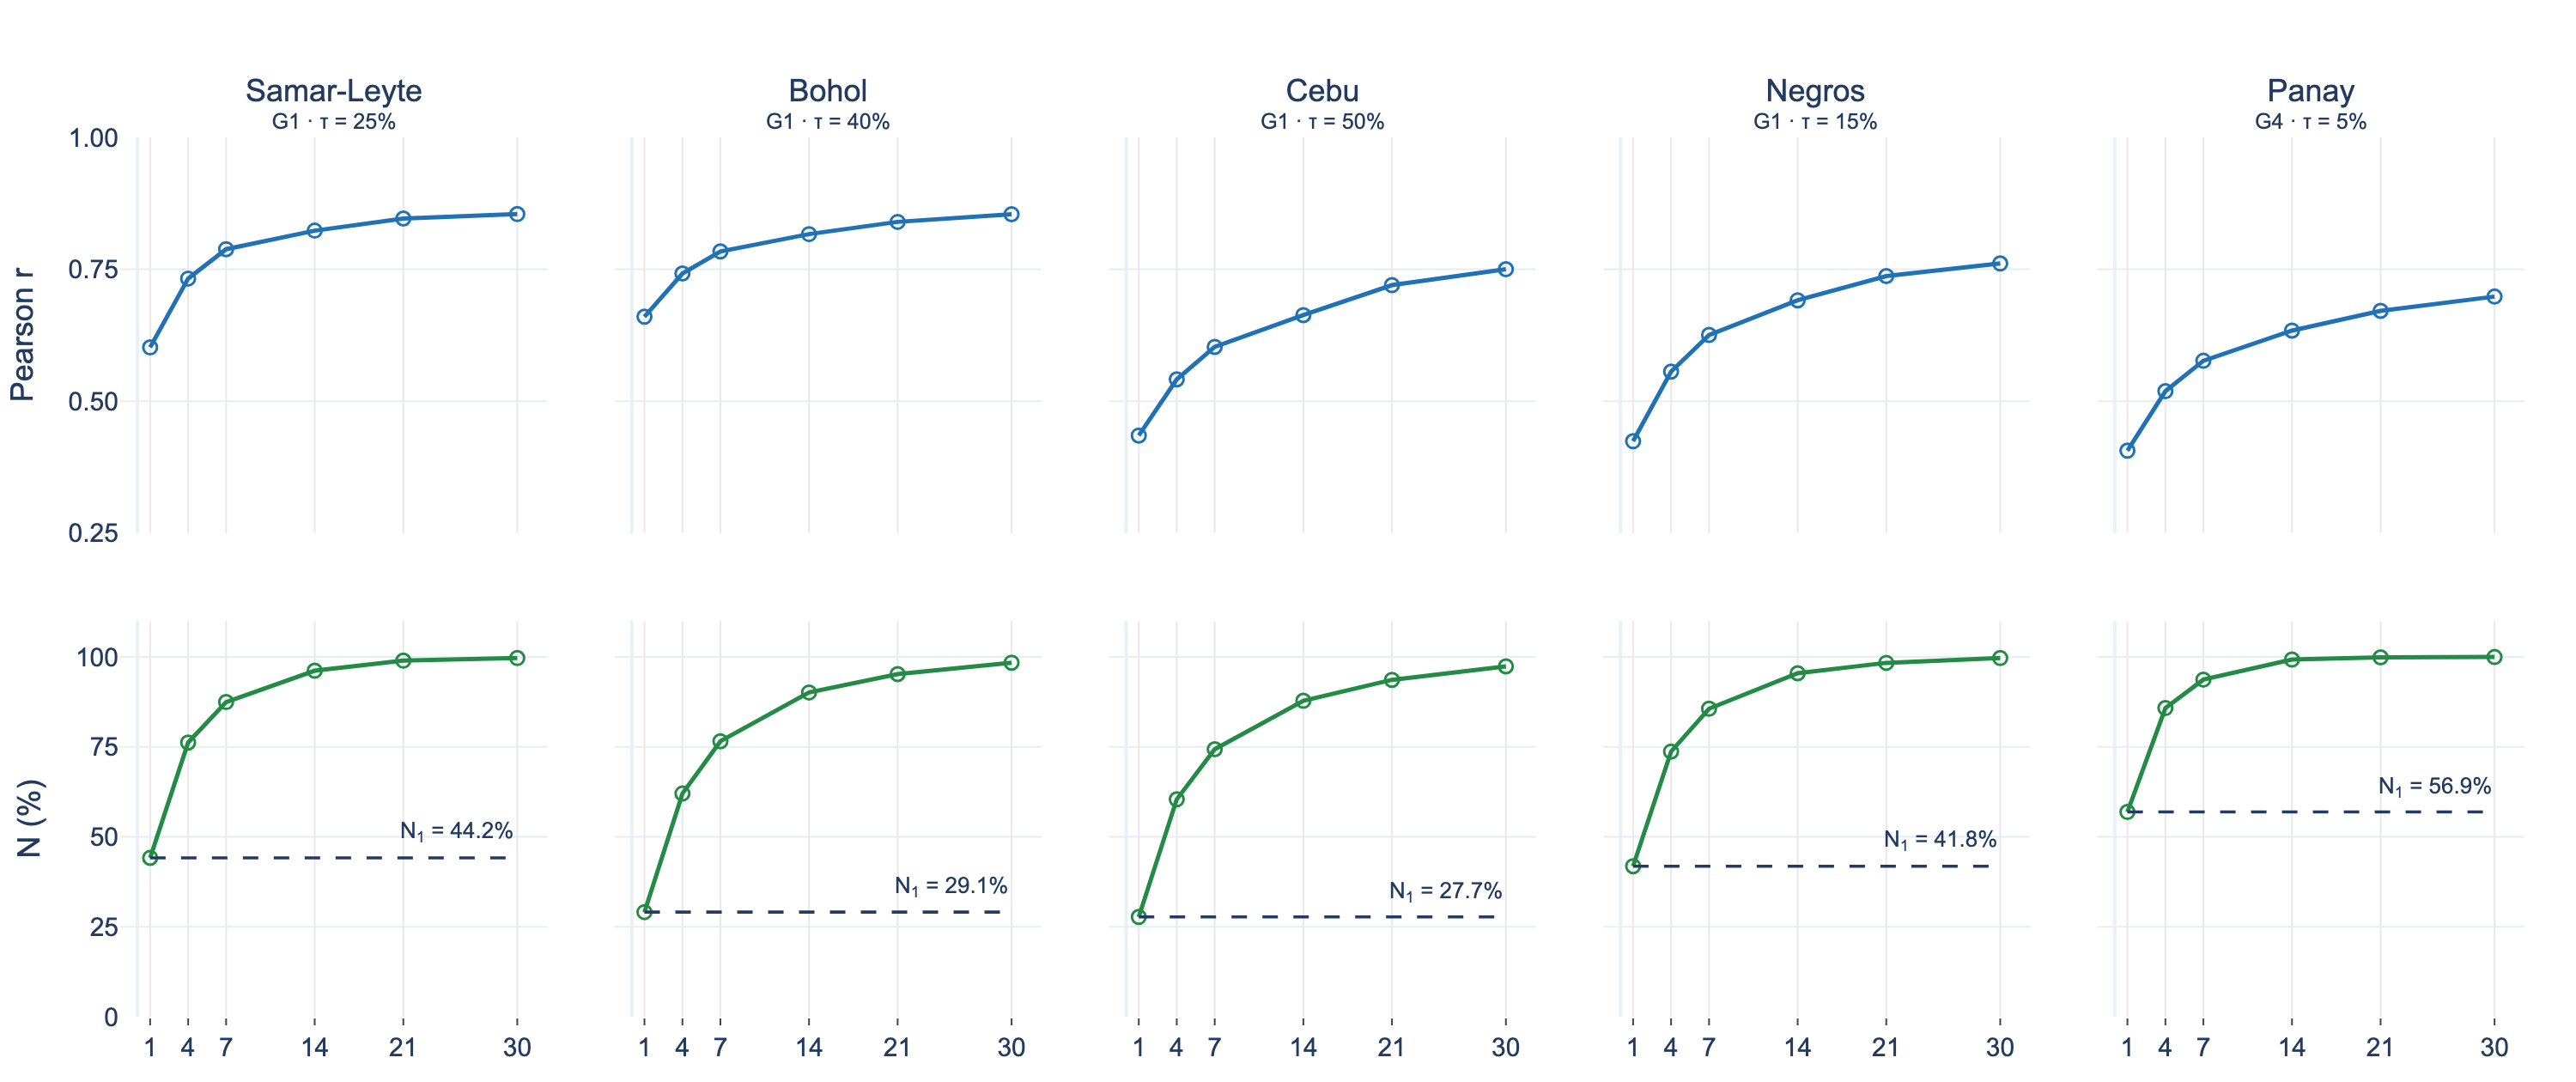
\includegraphics[width=\linewidth]{figs/fig_10_fixed_configuration_window_sensitivity.png}
        \caption{Sensitivity of NTL--load alignment to centred calendar window length at the configurations selected at $W=1$ for the five Visayas sub-grids. Upper panels show Pearson $r$ calculated on the same directly paired $W=1$ dates at every window length. In the lower panels, solid lines show paired-estimate availability and dashed lines show retained direct-date coverage at $W=1$. Both percentages use dates with an available NGCP load observation as the denominator. Paired-estimate availability requires both window means to be calculable, with at least one qualifying value per series within the window.}
        \label{fig:window_sensitivity}
    \end{figure*}
    
        Figure~\ref{fig:visayas_timeseries} shows the full-record and Rai-window alignment for the four configurations outlined in Figure~\ref{fig:regional_daily_heatmaps}. In the Rai window, the load decline and subsequent rise are most pronounced in Bohol and Cebu, where $r_1$ is 0.86 and 0.66, supported by 53 and 57 directly paired days, respectively. Negros and Panay show weaker correspondence, with $r_1$ of 0.16 and 0.17. Panay retains directly paired observations on 58\% of calendar days in the event window, compared with 22\% in Bohol and 24\% in Cebu. The trailing means show broader temporal patterns alongside the intermittent $W=1$ observations.
    
    \subsection{Sensitivity to Temporal Window Length}
        
        The effect of temporal averaging is evaluated with the mask and SC threshold held fixed at the configuration selected at $W=1$ for each sub-grid (Table~\ref{tab:transferability}). Figure~\ref{fig:window_sensitivity} shows Pearson $r$ and paired-estimate availability across centred calendar windows of 1, 4, 7, 14, 21, and 30 days. Within each sub-grid, correlations at all window lengths use the same directly paired dates identified at $W=1$.
        
        Pearson $r$ increases with window length in all five sub-grids. In Samar--Leyte, it rises from 0.602 at $W=1$ to 0.788 at $W=7$ and 0.855 at $W=30$. At $W=30$, correlations range from 0.698 in Panay to 0.855 in Samar--Leyte, with Bohol reaching a similar value of 0.854 (Supplementary Table~S5). The largest gains generally occur at shorter windows, followed by smaller increases towards 30 days.
        
        Paired-estimate availability also increases with window length, reaching 97.4--100\% at $W=30$. Bohol and Cebu show particularly large differences between estimate availability and direct-date coverage: fewer than 30\% of NGCP dates have a qualifying direct NTL observation, while more than 97\% have paired 30-day estimates. In Samar--Leyte, $W=14$ already yields $r=0.823$ and 96.2\% estimate availability. Extending the window to 30 days adds approximately 0.032 to $r$ and 3.5 percentage points to estimate availability, while direct-date coverage remains 44.2\% and the correlation sample remains fixed at 1,936 paired days.

\section{Discussion}
    
    \subsection{Observability as a Structural Constraint on Daily NTL Interpretation}
    
        The results show that daily VIIRS Black Marble observations in Samar--Leyte are highly intermittent across both POI and settlement scales. At city and municipal POIs, observations meeting the majority-support criterion are available on approximately one-third of calendar days, and increasing support from $1\times1$ to $5\times5$ pixels produces little improvement in admissible-day frequency (Table~\ref{tab:poi_summary}). Radiance variability can nevertheless decrease with kernel size (Figure~\ref{fig:poi_cv}). Spatial averaging and observational availability therefore respond differently to enlargement of the spatial support.
        
        This distinction is central to the reliability argument. Lower variability on retained days can coexist with prolonged intervals that fail the admissibility criterion. The POI-level results in Supplementary Table~S2 show why annual completeness and dropout duration need to be considered together: Palo and Alang-Alang have similar $TC_{50}$ values of approximately 35\% at $1\times1$, but their longest dropouts are 38 and 21 days. Their observation frequencies are similar, while their capacity to resolve a process occurring within those gaps differs substantially. Supplementary Figure~S5 adds the temporal placement of the gaps, identifying which portions of the radiance trajectory are supported by qualifying observations.
        
        The contrast between DNB-BRDF and gap-filled radiance further clarifies the difference between continuity and observability. Gap-filled series have lower temporal CV and smoother trajectories, including during intervals with sparse direct observations (Supplementary Figures~S1--S2 and~S5). Their continuity partly depends on values supplied across missing retrievals. Reduced variability consequently describes a change in signal representation; its value for a particular application depends on whether the reconstruction preserves the changes of interest. Retaining DNB-BRDF as the primary observational record keeps the distinction between direct support and reconstructed continuity visible throughout the framework.
        
        The long-term SC diagnostics in Supplementary Figure~S3 show that incomplete sampling is embedded within seasonal and interannual observation patterns across 2012--2024. The global TC map places the Philippine case within a wider pattern of low completeness across equatorial and monsoonal regions (Figure~\ref{fig:temporal_maps}). The nominal daily frequency of the product therefore needs to be interpreted alongside the actual frequency and continuity of surface observations. These properties determine the temporal evidence available before radiance changes are associated with an underlying process.
    
    \subsection{Settlement Structure Conditions the Reliability of NTL Signals}
    
        Settlement stratification substantially changes the signal being analysed. Urban centres and clusters occupy a small fraction of the Samar--Leyte domain, while non-urban cells comprise most of its area (Table~\ref{tab:settlement_grouped}). The individual-class series show stronger urban radiance alongside low-intensity rural and water backgrounds (Supplementary Figure~S6). Cumulative masks progressively combine these environments, changing the spatial target and the mixture of radiance contributing to its daily mean (Supplementary Figure~S7).
        
        Completeness and signal relevance consequently provide different information. Water retains a greater proportion of admissible dates than the urban-centre class, although its radiance remains close to background levels. Conversely, a brighter urban signal can still contain extended inadmissible intervals. The class-level CV values in Supplementary Table~S3 add a further distinction: relative variability depends on both dispersion and mean radiance. A low CV may describe a stable illuminated environment or a consistently dim background, while a small mean can magnify relative fluctuations. Availability and stability become informative for electricity-related interpretation when evaluated alongside the thematic content of the observed signal.
        
        Spatial support also conditions the magnitude of the change being summarised. The pre--post Haiyan contrasts in Supplementary Figure~S4 decrease in magnitude as the kernels incorporate a broader neighbourhood. This reflects a change in the spatial mixture represented by the estimate, alongside differences in available observations. Similarly, an admissible class mean describes support for the class-wide target and does not establish that every constituent location was observed. The spatial unit must therefore be defined before its completeness, variability, or radiance contrast is interpreted.
        
        The stronger alignment of urban-focused masks with NGCP load is consistent with the concentration of electricity-related lighting within those supports (Figures~\ref{fig:threshold_sweep} and~\ref{fig:alignment_25pct}). Broader masks incorporate additional low-emission environments and can retain more dates while exhibiting weaker correspondence. These comparisons identify spatial supports relevant to the observed load relationship. They leave the physical contributions of individual locations unresolved, particularly where aggregate demand and remotely observed lighting represent different parts of the electricity system.
    
    \subsection{Completeness Thresholds Define a Context-Dependent Trade-Off}
    
        The spatial completeness threshold changes both the support required for a daily estimate and the temporal sample entering the comparison. The 50\% criterion used for observability diagnostics provides a common reference for comparing kernels and classes. The alignment sweep then evaluates how alternative support requirements affect correspondence and retained coverage within each thematic mask. The selected threshold represents a working point under the stated ranking rule.
        
        The Samar--Leyte heatmaps show why stronger correlation alone is insufficient to identify that working point (Figure~\ref{fig:threshold_sweep}). Increasing the G1 threshold from 25\% to 40\% raises correlation while reducing retained coverage, resulting in a slightly lower composite score. The full-record and Haiyan comparisons in Supplementary Figures~S8--S9 also show that broad trajectories can persist across thresholds while local profiles and estimate availability change. Because SC varies through time, stricter thresholds can alter the seasonal and event-period composition of the retained sample. Changes in correlation therefore combine changes in required spatial support with changes in the dates being compared.
        
        The scoring sensitivity makes the selection preference explicit. Replacing the squared positive-correlation term with its linear alternative changes the selected configuration in four sub-grids (Supplementary Figure~S11). Agreement across a complete ranking can nevertheless remain high when its leading configuration changes. The distinction is important: similar rankings indicate a recurring pattern across candidates, while changes at the top identify settings sensitive to the relative emphasis placed on correspondence and retention.
        
        The near-tied Panay configurations provide a complementary example (Supplementary Table~S4 and Figure~S10). Similar scores arise from a broader urban support retaining many more dates and a narrower support with stronger correlation. These configurations offer different temporal samples and spatial representations. The score makes their comparison transparent, while the observability diagnostics remain necessary to assess gap placement and continuity for the period of interest. Reliability qualification thus links configuration ranking back to the observation sequences on which interpretation depends.
        
    \subsection{Regional Consistency Across Island Sub-Grids}
    
        The regional comparisons show a recurring preference for urban-focused supports, accompanied by variation in the selected footprint and threshold (Figure~\ref{fig:regional_daily_heatmaps}; Table~\ref{tab:transferability}). G1 Urban Core is selected in four sub-grids, while Panay selects G4 Urban Fringe. The Panay result is particularly informative because it shows that the useful spatial target can extend beyond the urban-centre class. Concentrated urban lighting provides a consistent candidate family across these experiments, but its most suitable extent varies between sub-grids.
        
        The expanded rankings in Supplementary Table~S4 show that neighbouring thresholds often produce similar scores within the same mask family. The score-form comparison further shows that the selected masks remain urban-focused under both rules, even where the precise mask and threshold change (Supplementary Figure~S11). Regional consistency is therefore strongest at the level of the settlement context represented by the signal. The exact operating point depends on the local observation record and the declared balance between correspondence and retention.
        
        The event enlargements also show that correspondence varies with the period evaluated (Figures~\ref{fig:alignment_25pct} and~\ref{fig:visayas_timeseries}). The Haiyan transition is more prominent than many shorter fluctuations in the full record, while the Rai window exhibits strong correspondence in Bohol and Cebu and weaker correspondence in Negros and Panay. Greater retained coverage in Panay does not produce the strongest event-period association. These differences reinforce the value of inspecting the observation sequence and reporting support for the displayed period, alongside the full-record configuration assessment.
    
    \subsection{Temporal Averaging Changes the Scale of Correspondence}
    
        The window-sensitivity analysis separates the effect of temporal averaging from changes in the correlation sample. With the selected spatial configurations and directly paired dates held fixed, correlation increases across all five sub-grids (Figure~\ref{fig:window_sensitivity}). In Samar--Leyte, the increase from 0.602 at $W=1$ to 0.855 at $W=30$ describes stronger agreement between temporally aggregated signals. Averaging suppresses some short-term differences and gives greater prominence to shared variation over longer periods. The resulting correspondence has a broader temporal meaning than the association evaluated at $W=1$.
        
        The accompanying increase in estimate availability has a separate interpretation. Samar--Leyte reaches 99.7\% paired-estimate availability at $W=30$, while direct-date coverage remains 44.2\% (Supplementary Table~S5). Overlapping windows reuse observations, and the minimum-support rule permits means based on different numbers of contributing dates. An almost complete sequence of estimates can therefore be supported by an intermittent and unevenly distributed direct record. Reporting $N_{\%}$ and $N_{\mathrm{est}}$ together exposes this dependence, which would be obscured by reporting the continuity of the averaged series alone.
        
        Window length consequently belongs to the definition of the signal used for interpretation. Previous applications have adopted different temporal supports for restoration assessment and urban change modelling \citep{Roman2019_PLOSone_Maria,Chakraborty2023_RSE_AdaptiveModeling}. The present sensitivity curves quantify how those choices affect correspondence and estimate availability within fixed spatial settings. Centred windows provide retrospective comparisons, while the trailing profiles in Supplementary Figures~S8--S9 show how earlier observations continue to contribute around a transition. A suitable window depends on the temporal detail required by the application and the observations available to support it. Maximising correlation alone would favour temporal aggregation without accounting for the shorter features being averaged.
    
    \subsection{Implications for Disaster Monitoring with Daily NTL}
    
        Prior work has demonstrated the value of Black Marble for electricity outage and restoration assessment, including after Hurricane Maria \citep{Roman2019_PLOSone_Maria}. The preliminary ISPRS study introduced the diagnostic-first concept and explored GHSL-based aggregation and completeness thresholds using temporally aggregated alignment \citep{Principe2026_ISPRS}. The present study extends that foundation by selecting configurations at $W=1$, testing sensitivity to the scoring rule, and evaluating temporal averaging on fixed directly paired dates. Together with the expanded POI, kernel, and settlement-class diagnostics, these analyses establish how the observational basis of the signal changes through the processing sequence.
        
        The resulting scientific contribution is the demonstrated interaction between spatial definition, admissibility, external correspondence, and temporal representation. A larger kernel can reduce variability while leaving observation frequency unchanged or increasing the longest gap. A stricter threshold can strengthen correspondence while removing parts of the temporal sequence. A longer window can strengthen correspondence and produce almost continuous estimates while retaining the same direct observational base. The ordered framework in Figure~\ref{fig:schematic} makes these outcomes traceable: each stage establishes conditions that remain relevant when the next decision is made.
        
        For disaster applications, this means identifying the evidence available around the transition being interpreted. A pre--post contrast may be supported by qualifying observations on either side of an event while its precise timing remains poorly constrained. A smooth recovery-shaped trajectory may also combine observations from different stages of that transition. Reporting the spatial target, qualifying dates, gap structure, and temporal window allows such distinctions to accompany downstream analysis. Reliability qualification provides an observational basis for deciding which features can be examined directly, which depend on temporal aggregation, and which remain unresolved within the available record.
        
    \subsection{Limitations and Future Directions}
    
        Long observation gaps and sparse qualifying dates constrain the temporal detail available for event assessment. Whole-record correlations can also include shared long-term trajectories and seasonal variation. Moreover, satellite radiance and sub-grid load describe different measurement targets: radiance reflects the illuminated surfaces observed from above, while load integrates electricity demand across the operational sub-grid. Their correspondence can vary with lighting practices, the distribution of electricity uses, and local generation. The alignment results characterise association within the evaluated spatial and temporal supports.
        
        The spatial masks retain the 2015 GHSL classification throughout 2012--2024, maintaining consistent reference footprints. Expansion, densification, and land-cover conversion can alter conditions within those footprints, while the valid-pixel membership changes with retrieval availability. Cumulative masks broaden the settlement environments included but retain the same reference epoch. Alignment thresholds are also conditional on the observed-maximum valid-pixel normalisation, the analysis record, and the adopted quality and radiance screening.
        
        Geographical evaluation is restricted to five related Visayas sub-grids. The global TC map provides geographical context for observation constraints, while the alignment experiments establish regional evidence within those sub-grids. Configuration selection on the evaluation record introduces potential selection optimism. Haiyan and Rai provide event-period illustrations, but correspondence around known landfalls does not establish detection accuracy or recovery-estimation performance against independently labelled events.
        
        Further evaluation should use temporally separated selection and assessment, additional geographical and climatic settings, and sensitivity tests for the GHSL reference epoch and updated classifications. Adaptive admissibility rules offer another direction, provided that their effects on spatial support and temporal retention remain explicit. Benchmarking against independent outage records would then establish how reliability qualification affects event detection and recovery estimation.
                                
\section{Conclusion}

    
    Daily NASA Black Marble observations in humid tropical regions are frequently interrupted by cloud-driven gaps. In Samar--Leyte, intervals without observations meeting the spatial-support criterion reach 39 days. Larger neighbourhoods reduce some radiance variability while these interruptions largely persist. A more stable radiance series can therefore provide a clearer view of broad change without resolving the missing portions of its history.
    
    The reliability-qualified NTL framework connects this observational context to the construction and interpretation of the signal. Across five Visayas sub-grids, GHSL-based spatial qualification favours urban-focused supports, with daily correlations of $r=0.406$--$0.660$ supported by 27.7--56.9\% retained coverage. Selected completeness thresholds range from 5\% to 50\%, while sensitivity tests show how ranking and averaging choices change the resulting representation. These findings establish that the spatial target, retained observations, and analysis timescale jointly determine what electricity-related information can be drawn from daily NTL.
    
    The principal contribution is a systematic diagnostic framework for making those dependencies explicit before impact or recovery metrics are applied. It provides a common basis for evaluating both event-period and long-record interpretations while accommodating their different spatial and temporal requirements. Metrics developed under better-observed conditions can then be assessed against the evidence available in cloud-limited settings. This gives daily NTL a clearer role in disaster research: supporting interpretation at the scales justified by its observations, with the remaining gaps carried forward as part of the evidence.

    \section*{Acknowledgements}
    
    Rene Jr. L. Principe acknowledges support from the RMIT Research Stipend Scholarship (RRSS) and the RMIT International Tuition Fee Scholarship (RRITFS). The authors gratefully acknowledge the School of Science at RMIT University for providing computational resources and research infrastructure that supported this work.

    During preparation of this manuscript, the authors used ChatGPT (OpenAI) to assist with language refinement, LaTeX formatting, and code readability. All AI-assisted content was reviewed and verified by the authors, who take full responsibility for the accuracy and integrity of the final manuscript.
    
    \section*{Disclosure statement}
    
    The authors declare that they have no known competing financial interests or personal relationships that could have appeared to influence the work reported in this paper.
    
    \section*{Funding}
    
    This research is funded and supported by a Postgraduate Scholarship from Natural Hazards Research Australia.
    
    \section*{Data availability statement}
    
    Processed data and analysis outputs supporting this study are openly available on Zenodo at
    \url{https://doi.org/10.5281/zenodo.21051901} \citep{Principe2026_Data}.
    The reproducible code, including Google Earth Engine scripts, Python workflows, notebooks, and documentation, is archived with the Zenodo release.
    
    NASA Black Marble VNP46A2 and GHSL-SMOD source data are available from their official repositories and are not redistributed. Hourly electricity-demand data were obtained from the publicly accessible National Grid Corporation of the Philippines
    Operations portal. Original NGCP files are not redistributed; derived analysis-ready variables and processing documentation are provided subject to the source provider's reuse conditions.
    
    \section*{CRediT authorship contribution statement}
    
    \textbf{Rene Jr. L. Principe:} Conceptualization, Methodology, Software, Validation, Formal analysis, Investigation, Visualization, Writing -- original draft, Writing -- review and editing. \textbf{Karin Reinke:} Supervision, Formal analysis, Investigation, Writing -- review and editing, Project administration. \textbf{Simon Jones:} Supervision, Formal analysis, Writing -- review and editing, Project administration.


\bibliographystyle{tfcad}
\bibliography{interactcadsample}


\end{document}
